%%%%%%%%%%%%%%%%%%%%%%%%%%%%%%%%%%%%%%%%%%%%%%%%%%%%%%%%%%%%%%%%%%%%%%%%
%                                                                      %
%     File: Thesis_Evaluation.tex                                         %
%     Tex Master: Thesis.tex                                           %
%                                                                      %
%     Author: Andre C. Marta                                           %
%     Last modified :  2 Jul 2015                                      %
%                                                                      %
%%%%%%%%%%%%%%%%%%%%%%%%%%%%%%%%%%%%%%%%%%%%%%%%%%%%%%%%%%%%%%%%%%%%%%%%

\chapter{Evaluation}
\label{chapter:evaluation}

%%%%%%%%%%%%%%%%%%%%%%%%%%%%%%%%%%%%%%%%%%%%%%%%%%%%%%%%%%%%%%%%%%%%%%%%
\section{Test Methodology}
\label{section:test-methodology}

We implemented our CRSH algorithm in OpenGL/C++ and CUDA/C++ then compared it with our implementation of RAH \cite{Roger07} over the same architecture. We map our algorithm onto the GPU, parallelizing it there fully. We achieve this mainly by the use of parallel primitives, like prefix sums \cite{Blelloch90}. We used the CUB \cite{Merrill09}  \cite{Merrill11} library to perform parallel radix sorts and prefix sums.

\medskip

We measure the amount of intersections, including misses and hits, to evaluate ray hierarchy algorithms proficiency at reducing the amount of ray-primitive intersection tests required to render an image. All scenes were rendered at $512\times512$ resolution. We also vary the depth of the hierarchy and the number of nodes we combine to create the upper levels of the hierarchy. We also measured the frame rate of each scene using a baseline configuration as well as the individual steps in each algorithm relatively to the overall frame rate.

\medskip

The test information was collected using a NVIDIA GeForce GTX TITAN GPU with 6 GB of RAM. Our algorithm is completely executed on the GPU (including hierarchy construction and traversal) so the CPU has no impact on the test results.

%%%%%%%%%%%%%%%%%%%%%%%%%%%%%%%%%%%%%%%%%%%%%%%%%%%%%%%%%%%%%%%%%%%%%%%%
\section{Test Scenes}
\label{section:test-scenes}

We used three different scenes, \textsc{Office}, \textsc{Cornell} and \textsc{Sponza}.

\medskip

The \textsc{Office} scene (36K triangles) is representative of interior design applications. It is divided into several submeshes therefore it adapts very well to our bounding volume scheme. For this scene the emphasis was on testing shadow rays. 

\medskip

We selected \textsc{Cornell} (790 triangles). as it is representative of highly reflective scenes. It consists an object surrounded by six mirrors. On this scene we focused on testing reflection rays although it also features shadow rays in it.

\medskip

\textsc{Sponza} (66K triangles), much like \textsc{Office}, is representative of architectural scenes. For this scene the emphasis was also on testing shadow rays but for scenes that do not conform with our bounding volume scheme. This scene does not adapt well to our scheme as is not divided into submeshes. 

%%%%%%%%%%%%%%%%%%%%%%%%%%%%%%%%%%%%%%%%%%%%%%%%%%%%%%%%%%%%%%%%%%%%%%%%
\section{Test Hypothesis}
\label{section:test-hypothesis}

We hypothesised that our more coherent RSH hierarchy needs to compute fewer intersection results to render a scene. We expect more expressive results for shadow rays. As shadow rays have low divergence the sorting step should create a more coherent RSH than for reflection rays. In addition our hierarchy should also be more coherent with reflection rays than one based on the RAH algorithm due to the hashing we use. However by the very nature of reflection rays they will never be as coherent as shadow rays resulting in a lower quality hierarchy.

By varying the depth of the hierarchy we also expect that with hierarchies of a certain depth the upper nodes in the hierarchy will have degenerated so much that processing them leads to no benefit at all. In other words, these nodes will be so wide that they will intersect all the geometry in the scene, which means that we just wasted time processing them since we didn't prevent any future intersection tests. This should happen because as we go up in the hierarchy the nodes will encompass so many rays that they will be too large.

By varying the number of nodes used to create the upper levels of the hierarchy we expect a similar outcome to varying the depth. If we use more lower level nodes to create the upper level ones, the upper level nodes will be larger therefore after a certain level they will be too wide (i.e using 16 level 0 nodes to create a level 1 node). However there is a trade-off related to the memory consumption of the algorithm. If we use more nodes to create the upper nodes we will have less nodes overall and thus need less memory to store the potential intersection hits.

\vskip 27em

\pagebreak

\def\arraystretch{1.5}%  1 is the default, change whatever you need

%%%%%%%%%%%%%%%%%%%%%%%%%%%%%%%%%%%%%%%%%%%%%%%%%%%%%%%%%%%%%%%%%%%%%%%%%%%%%%%%%%%%%%%%%%%%%%%%%%%%%%%%%%%%%%%%%%%%%%%%%%%%%%%%%%
\section{Test Results and Discussion}
\label{section:test-results-and-discussion}

\subsection{Hierarchy Traversal Results - Subdivision 8 Depth 2}

\subsubsection{Office}

% Office Discussion

Comparing our algorithm with the RAH algorithm we can see that our algorithm computes 63,79\% less intersections than RAH on this scene. 98,14\% less than a brute force approach (see Table~\ref{table:office-d8-n2-results} and Table~\ref{table:results-d8-n2}).

% Office Table and Figure
    
\begin{figure}[!htb]
    \begin{minipage}{0.25\linewidth}
        \centering
        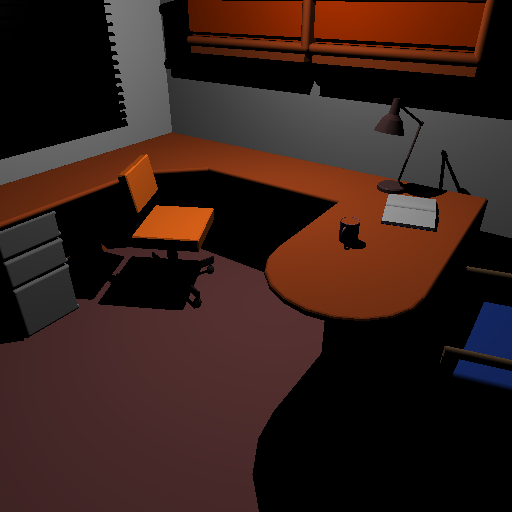
\includegraphics[width=4.0cm]{Images/Office_Preview}
        \captionof{figure}{\textsc{Office}}
    \end{minipage}
    \begin{minipage}{0.725\linewidth}
        \centering
        \fontencoding{T1}
        \fontseries{m}
        \fontshape{sc}
        \fontsize{8}{10}
        \selectfont
        \begin{tabular}[h]{l|rr}
            \multicolumn{1}{c|}{\textsc{Office}} & \textsc{Level 2} & \textsc{Level 1}\\
            \hline
            \emph{RAH Algorithm} & & \\
            \hline
            \quad \# Sh Intersections  & 142726748  & 202025920 \\
            \quad \# Sh Misses            & 117473508  & 186409563 \\
            \quad \# Sh Hits              & 25253240   & 15616357  \\
            \hline
            \emph{Our Algorithm} & & \\
            \hline
            \quad \# Sh Intersections  & 11559388   & 85572416	\\
            \quad \# Sh Misses         & 862836     & 76455023  \\
            \quad \# Sh Hits           & 10696552   & 9117393   \\
        \end{tabular}
        \label{table:office-d8-n2-results}
        \captionof{table}{\textsc{Office} Division 8 Depth 2 Test Results.}
    \end{minipage}
\end{figure}

\subsubsection{Cornell}

% Cornel Discussion

Comparing our algorithm with the RAH algorithm we can see that our algorithm computes 26,47\% less intersections than RAH on this scene. 91,17\% less than a brute force approach (see Table~\ref{table:cornell-d8-n2-results} and Table~\ref{table:results-d8-n2}).

% Cornell Table and Figure

\begin{figure}[!htb]
    \begin{minipage}{0.25\linewidth}
        \centering
        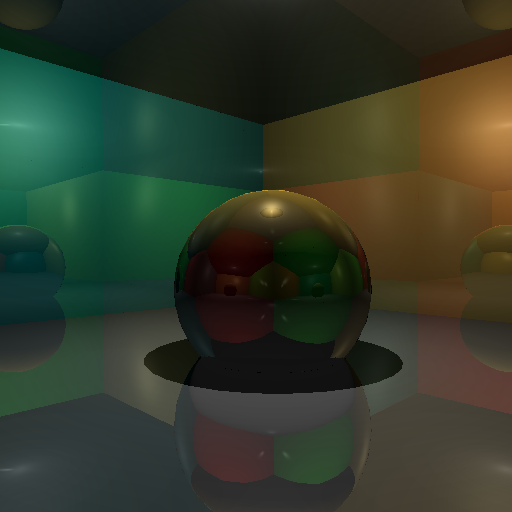
\includegraphics[width=4.0cm]{Images/Cornell_Preview}
        \captionof{figure}{\textsc{Cornell}}
    \end{minipage}
    \begin{minipage}{0.725\linewidth}
        \centering
        \fontencoding{T1}
        \fontseries{m}
        \fontshape{sc}
        \fontsize{8}{10}
        \selectfont
        \begin{tabular}[h]{l|rr}
            \multicolumn{1}{c|}{\textsc{Office}} & \textsc{Level 2} & \textsc{Level 1}\\
            \hline
            \emph{RAH Algorithm} & & \\
            \hline
            \quad \# Sh Intersections   & 2995344   & 5167632		  \\
            \quad \# Sh Misses             & 2349390   & 3606077		  \\
            \quad \# Sh Hits               & 645954    & 1561555		  \\
            & & \\
            \quad \# Re Intersections   & 6488064   & 17802296		  \\
            \quad \# Re Misses             & 4262777   & 14311812		  \\
            \quad \# Re Hits               & 2225287   & 3490484		  \\
            \hline
            \emph{Our Algorithm} & & \\
            \hline
            \quad \# Sh Intersections   & 750384    & 2375896		  \\
            \quad \# Sh Misses          & 453397    & 981144		  \\
            \quad \# Sh Hits            & 296987	& 1394752  	      \\
            & & \\
            \quad \# Re Intersections   & 2737872   & 10269256		  \\
            \quad \# Re Misses             & 1454215   & 6983410		  \\
            \quad \# Re Hits               & 1283657   & 3285846   	  \\            
        \end{tabular}
        \label{table:cornell-d8-n2-results}
        \captionof{table}{\textsc{Cornell} Division 8 Depth 2 Test Results.}
    \end{minipage}
\end{figure}

\subsubsection{Sponza}

% Sponza Discussion

Comparing our algorithm with the RAH algorithm we can see that our algorithm computes 35,86\% less intersections than RAH on this scene. 97,62\% less than a brute force approach (see Table~\ref{table:sponza-d8-n2-results} and Table~\ref{table:results-d8-n2}).

% Sponza Table and Figure

\begin{figure}[!htb]
    \begin{minipage}{0.25\linewidth}
        \centering
        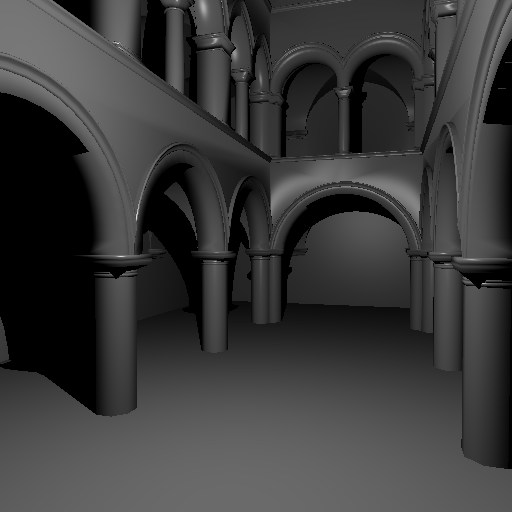
\includegraphics[width=4.0cm]{Images/Sponza_Preview}
        \captionof{figure}{\textsc{Sponza}}
    \end{minipage}
    \begin{minipage}{0.725\linewidth}
        \centering
        \fontencoding{T1}
        \fontseries{m}
        \fontshape{sc}
        \fontsize{8}{10}
        \selectfont
        \begin{tabular}[h]{l|rr}
            \multicolumn{1}{c|}{\textsc{Office}} & \textsc{Level 2} & \textsc{Level 1}\\
            \hline
            \emph{RAH Algorithm} & & \\
            \hline
            \quad \# Sh Intersections  & 266597400	& 261494752	  \\
            \quad \# Sh Misses            & 233910556  & 248455163	  \\
            \quad \# Sh Hits              & 32686844	& 13039589	  \\
            & & \\
            \hline
            \emph{Our Algorithm} & & \\
            \hline
            \quad \# Sh Intersections   & 266597400 & 62665496	  \\
            \quad \# Sh Misses          & 258764213 & 53120871	  \\
            \quad \# Sh Hits            & 7833187	& 9544625	  \\
        \end{tabular}
        \label{table:sponza-d8-n2-results}
        \captionof{table}{\textsc{Sponza} Division 8 Depth 2 Test Results.}
    \end{minipage}
\end{figure}

\subsection{Hierarchy Traversal Discussion - Subdivision 8 Depth 2}

% Comparison Table

\begin{table}[!htb]
    \begin{center}
    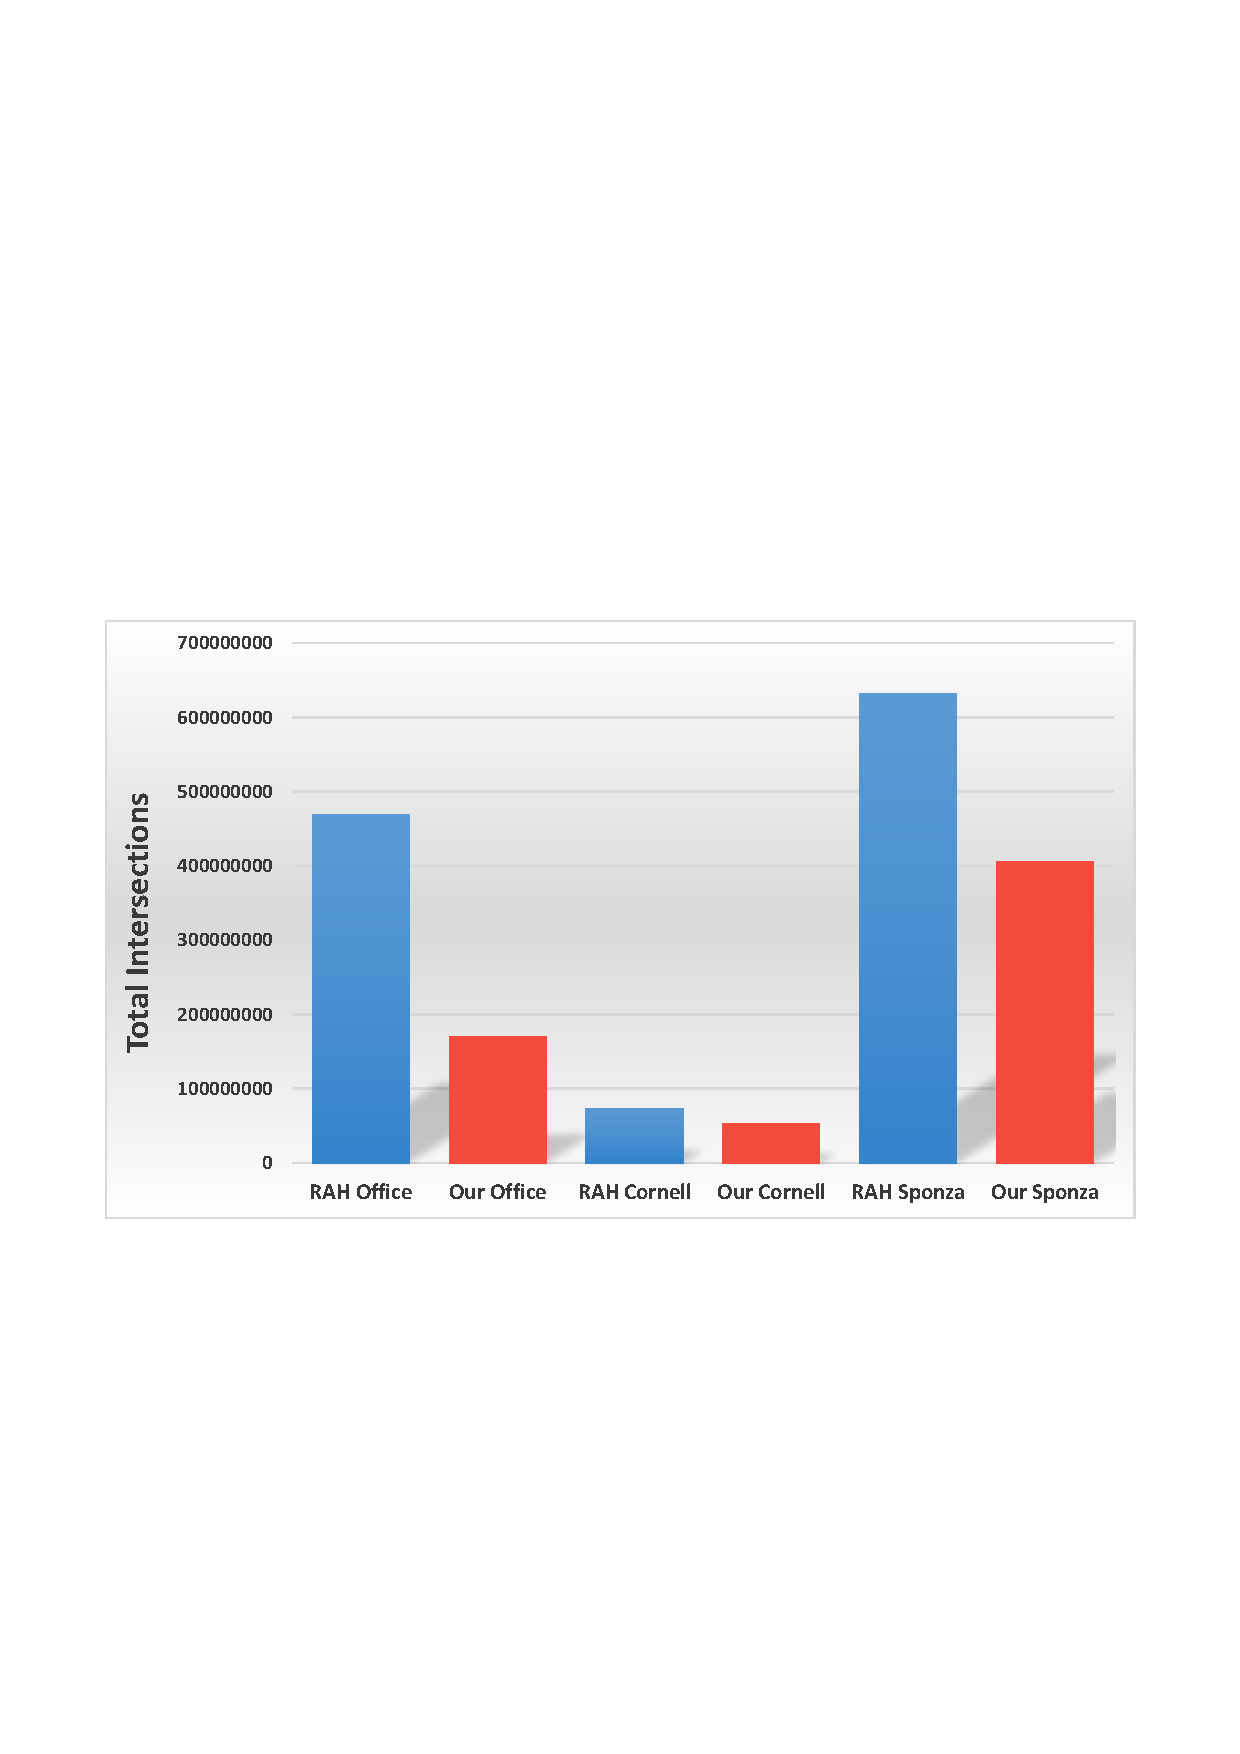
\includegraphics[width=0.85\textwidth]{Images/Chart_N8_D2}
    \vskip 2em
    \fontencoding{T1}
    \fontseries{m}
    \fontshape{sc}
    \fontsize{8}{10}
    \selectfont
    \begin{tabular}{l|rrrrrr}
    & \multicolumn{2}{c}{\textsc{Office}} & \multicolumn{2}{c}{\textsc{Cornell}} & \multicolumn{2}{c}{\textsc{Sponza}} \\
    \textsc{Algorithm} & \textsc{Total \# isect} & \textsc{Relative \%} & \textsc{Total \# isect} & \textsc{Relative \%} & \textsc{Total \# isect} & \textsc{Relative \%} \\
        \hline
        \emph{Brute Force}     & 9133132168         & 100\%           & 606911976         & 100\%           & 17058578850        & 100\% \\
        \emph{RAH Algorithm}   & 469683524		    & 5.14\%          & 72869648		  & 12.01\%         & 632408864			 & 3.71\% \\
        \emph{Our Algorithm}   & \textbf{170070948} & \textbf{1.86\%} & \textbf{53578192} & \textbf{8.83\%} & \textbf{405619896} & \textbf{2.38\%} \\
    \end{tabular}
    \end{center}
    \caption{\label{table:results-d8-n2}
    \small\textsc{Office} (251546 shadow rays), \textsc{Cornell} (242015 shadow \& 524288 reflection rays), \textsc{Sponza} (256713 shadow rays)  rendering performance using node subdivision 8 and hierarchy depth 2.}
\end{table}

For this set of tests we used a node subdivision of 8 and a hierarchy depth of 2. This means that every node in the upper levels of the hierarchy consists of 8 nodes in the level directly below (or 8 rays if we're constructing the first level of the hierarchy).

\subsubsection{Office}

Our initial expectations for Office were to get a much lower number of intersection tests with our algorithm than with RAH. The scene is a good fit to our bounding volume scheme and our highly coherent shadow ray hierarchy. Results confirm (see Table~\ref{table:office-d8-n2-results}) our initial expectations: we compute 63,79\% less intersections than RAH on this scene. 98,14\% less than a brute force approach.

\subsubsection{Cornell}

For the Cornell scene we focused primarily on the reflection rays which are much more incoherent than shadow rays so we expected results to be less positive than with the Office scene. We compute 26,47\% less intersections overall (shadow and reflection rays combined) than the RAH algorithm and 91,17\% less than the brute force approach (see Table~\ref{table:cornell-d8-n2-results}).

\subsubsection{Sponza}

The final scene, Sponza, is a whole mesh. We did not employ object subdivision in this scene. Hence we expected worse results than with Office since we would only get the benefit of the shadow ray hierarchy and none from the bounding volume scheme. We compute 35,86\% less intersection tests than RAH and 97,62\% than the brute force approach (see Table~\ref{table:sponza-d8-n2-results}). This confirmed our expectations since the results are about 50\% worse than they were with the Office. 

However even without the object subdivision our algorithm still manages to outperform RAH, which is very positive since these results all stem from the sorting we applied on the rays before creating the hierarchy.

\subsubsection{Configuration Comparison}

Since we have not analyzed the results for different subdivision and depth configurations we will only compare this setup (as a baseline) with the remaining ones in the next sections.

\vskip 15em

%%%%%%%%%%%%%%%%%%%%%%%%%%%%%%%%%%%%%%%%%%%%%%%%%%%%%%%%%%%%%%%%%%%%%%%%%%%%%%%%%%%%%%%%%%%%%%%%%%%%%%%%%%%%%%%%%%%%%%%%%%%%%%%%%%

\pagebreak
\subsection{Hierarchy Traversal Results - Subdivision 8 Depth 3}

\subsubsection{Office}

% Office Discussion

Comparing our algorithm with the RAH algorithm we can see that our algorithm computes 39,18\% less intersections than RAH on this scene. 97,87\% less than a brute force approach (see Table~\ref{table:office-d8-n3-results} and Table~\ref{table:results-d8-n3}).

% Office Table and Figure
    
\begin{figure}[!htb]
    \begin{minipage}{0.25\linewidth}
        \centering
        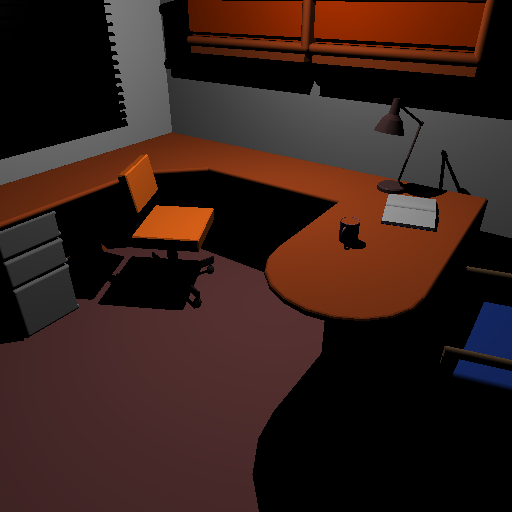
\includegraphics[width=4.0cm]{Images/Office_Preview}
        \captionof{figure}{\textsc{Office}}
    \end{minipage}
    \begin{minipage}{0.725\linewidth}
        \centering
        \fontencoding{T1}
        \fontseries{m}
        \fontshape{sc}
        \fontsize{8}{10}
        \selectfont
        \begin{tabular}[h]{l|rrr}
            \multicolumn{1}{c|}{\textsc{Office}} & \textsc{Level 3} & \textsc{Level 2} & \textsc{Level 1}\\
            \hline
            \emph{RAH Algorithm} & & \\
            \hline
            \quad \# Sh Intersections  & 17863536	& 131228368	& 202025920	\\
            \quad \# Sh Misses            & 1459990	& 105975128	& 186409563	\\
            \quad \# Sh Hits              & 16403546	& 25253240	& 15616357	\\
            \hline
            \emph{Our Algorithm} & & \\
            \hline
            \quad \# Sh Intersections  & 4108164    & 31864128	& 85755984	\\
            \quad \# Sh Misses         & 125148		& 21144630	& 76679022	\\
            \quad \# Sh Hits           & 3983016	& 10719498	& 9076962	\\
        \end{tabular}
        \label{table:office-d8-n3-results}
        \captionof{table}{\textsc{Office} Division 8 Depth 3 Test Results.}
    \end{minipage}
\end{figure}

\subsubsection{Cornell}

% Cornel Discussion

Comparing our algorithm with the RAH algorithm we can see that our algorithm computes 26,47\% less intersections than RAH on this scene. 91,17\% less than a brute force approach (see Table~\ref{table:cornell-d8-n3-results} and Table~\ref{table:results-d8-n3}).

% Cornell Table and Figure

\begin{figure}[!htb]
    \begin{minipage}{0.25\linewidth}
        \centering
        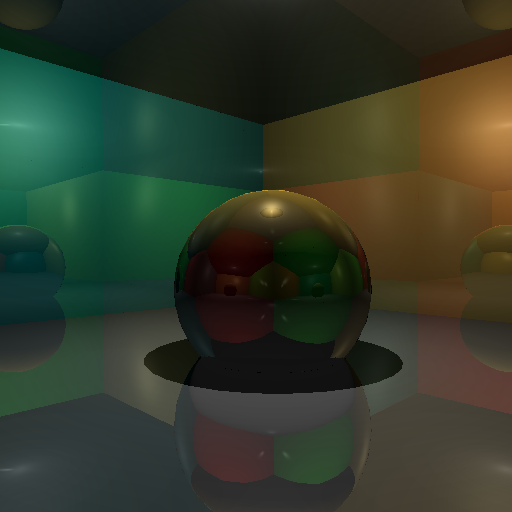
\includegraphics[width=4.0cm]{Images/Cornell_Preview}
        \captionof{figure}{\textsc{Cornell}}
    \end{minipage}
    \begin{minipage}{0.725\linewidth}
        \centering
        \fontencoding{T1}
        \fontseries{m}
        \fontshape{sc}
        \fontsize{8}{10}
        \selectfont
        \begin{tabular}[h]{l|rrr}
            \multicolumn{1}{c|}{\textsc{Office}} & \textsc{Level 3} & \textsc{Level 2} & \textsc{Level 1}\\
            \hline
            \emph{RAH Algorithm} & & \\
            \hline
            \quad \# Sh Intersections   & 374616 & 2617976 & 5156880    \\
            \quad \# Sh Misses             & 47369	 & 1973366 & 3606077    \\
            \quad \# Sh Hits               & 327247 & 644610  & 1550803    \\
            & & \\
            \quad \# Re Intersections   & 811008 & 6477632 & 17802296   \\
            \quad \# Re Misses             & 1304	 & 4252345 & 14311812   \\
            \quad \# Re Hits               & 809704 & 2225287 & 3490484    \\
            \hline
            \emph{Our Algorithm} & & \\
            \hline
            \quad \# Sh Intersections   & 181656 & 807208  & 2366280	\\
            \quad \# Sh Misses          & 80755	 & 511423  & 991955		\\
            \quad \# Sh Hits            & 100901 & 295785  & 1374325	\\
            & & \\
            \quad \# Re Intersections   & 614052 & 4143408 & 10278344	\\
            \quad \# Re Misses             & 96126	 & 2858615 & 6992777	\\
            \quad \# Re Hits               & 517926 & 1284793 & 3285567	\\            
        \end{tabular}
        \label{table:cornell-d8-n3-results}
        \captionof{table}{\textsc{Cornell} Division 8 Depth 3 Test Results.}
    \end{minipage}
\end{figure}

\subsubsection{Sponza}

% Sponza Discussion

Comparing our algorithm with the RAH algorithm we can see that our algorithm computes 35,86\% less intersections than RAH on this scene. 97,62\% less than a brute force approach (see Table~\ref{table:sponza-d8-n3-results} and Table~\ref{table:results-d8-n3}).

% Sponza Table and Figure

\begin{figure}[!htb]
    \begin{minipage}{0.25\linewidth}
        \centering
        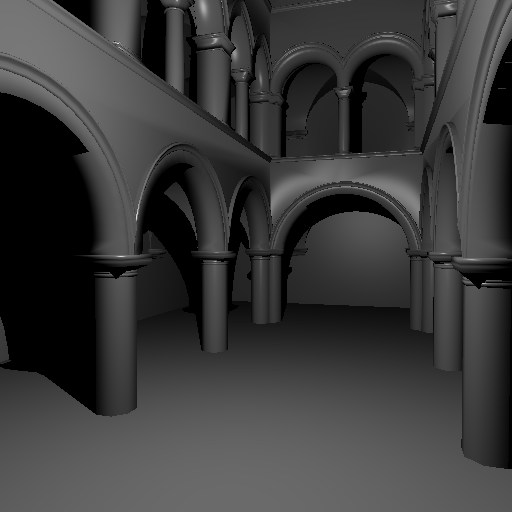
\includegraphics[width=4.0cm]{Images/Sponza_Preview}
        \captionof{figure}{\textsc{Sponza}}
    \end{minipage}
    \begin{minipage}{0.725\linewidth}
        \centering
        \fontencoding{T1}
        \fontseries{m}
        \fontshape{sc}
        \fontsize{8}{10}
        \selectfont
        \begin{tabular}[h]{l|rrr}
            \multicolumn{1}{c|}{\textsc{Office}} & \textsc{Level 3} & \textsc{Level 2} & \textsc{Level 1}\\
            \hline
            \emph{RAH Algorithm} & & \\
            \hline
            \quad \# Sh Intersections  & 33357900   & 214961944	& 261132816	\\
            \quad \# Sh Misses            & 6487657	& 182320342	& 248455163	\\
            \quad \# Sh Hits              & 26870243	& 32641602	& 12677653	\\
            & & \\
            \hline
            \emph{Our Algorithm} & & \\
            \hline
            \quad \# Sh Intersections   & 33357900	& 23359968	& 61887672	\\
            \quad \# Sh Misses          & 30437904	& 15624009	& 53120871	\\
            \quad \# Sh Hits            & 2919996	& 7735959	& 8766801	\\
        \end{tabular}
        \label{table:sponza-d8-n3-results}
        \captionof{table}{\textsc{Sponza} Division 8 Depth 3 Test Results.}
    \end{minipage}
\end{figure}

\subsection{Hierarchy Traversal Discussion - Subdivision 8 Depth 3}

% Comparison Table

\begin{table}[!htb]
    \begin{center}
    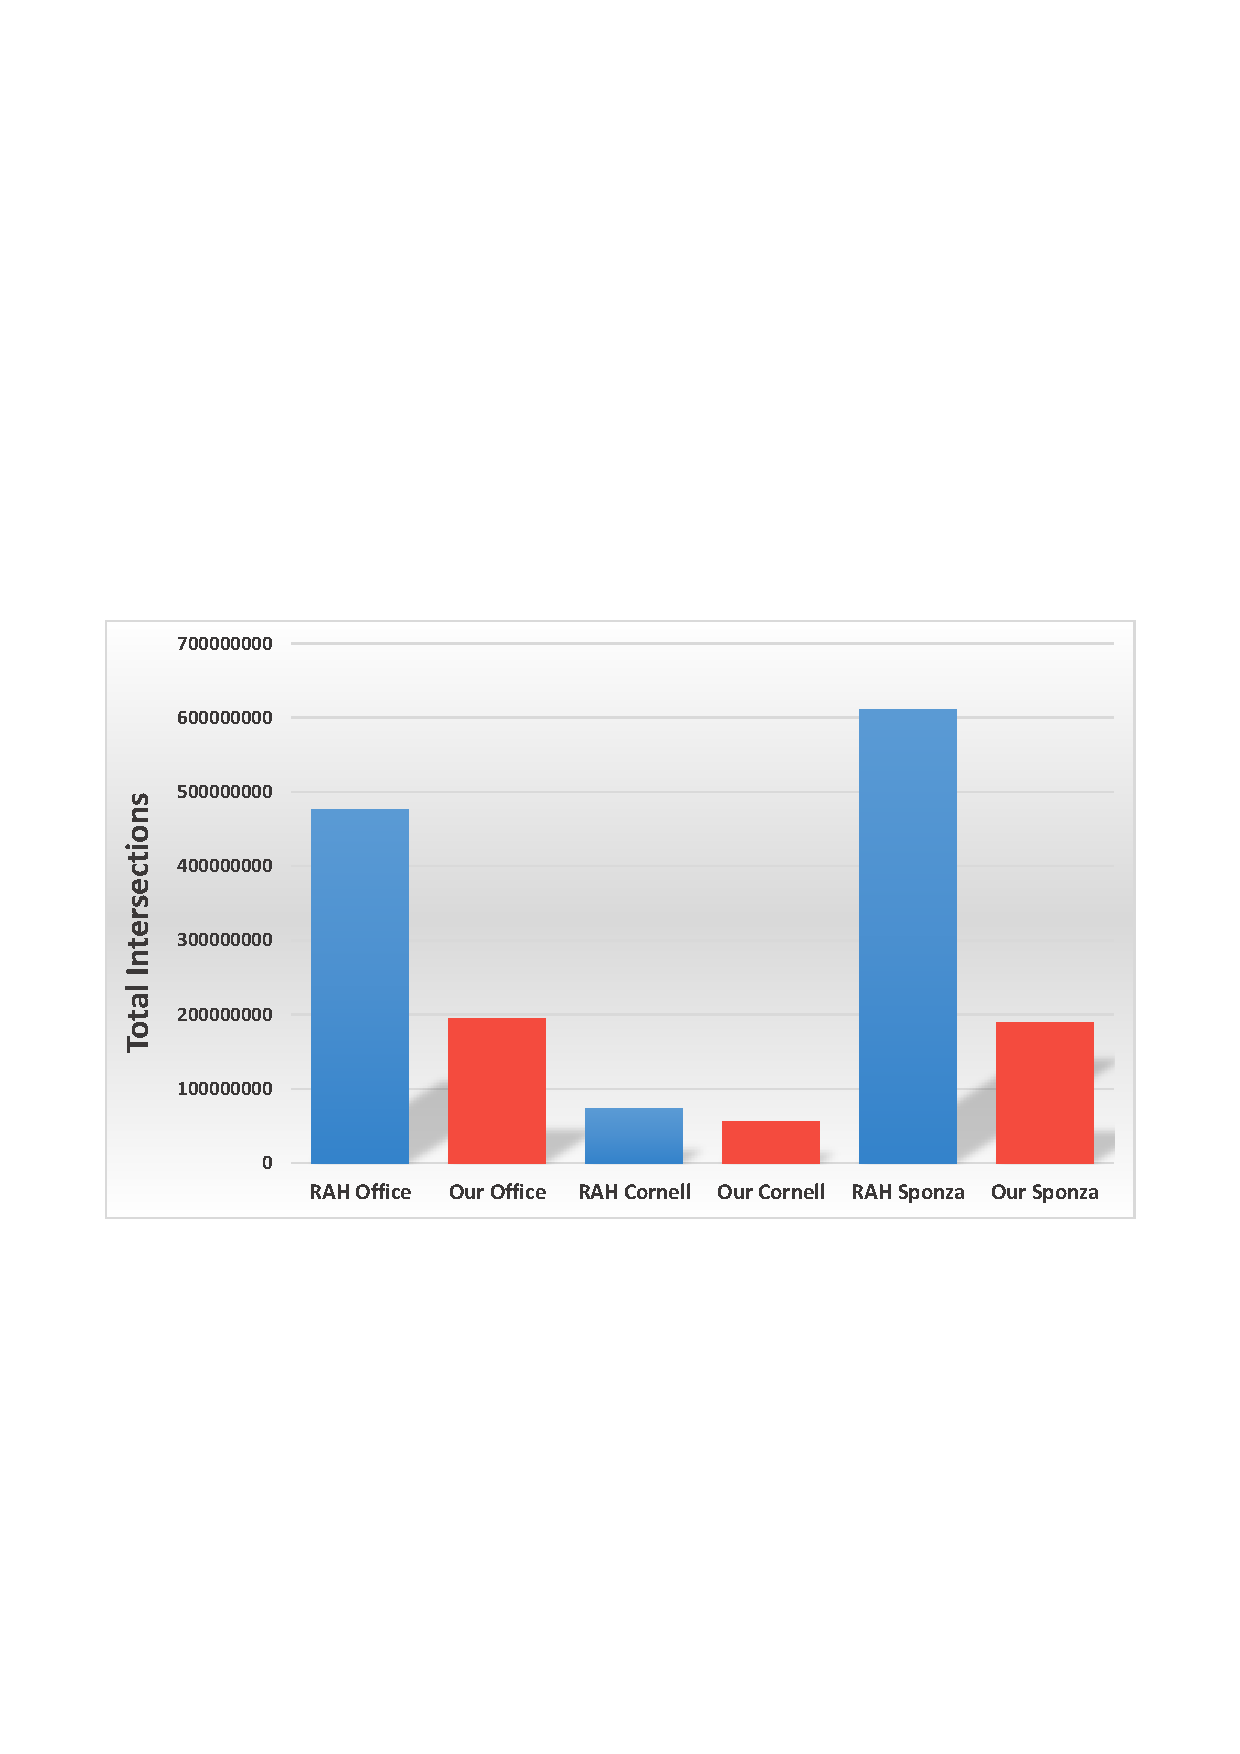
\includegraphics[width=0.85\textwidth]{Images/Chart_N8_D3}
    \vskip 2em
    \fontencoding{T1}
    \fontseries{m}
    \fontshape{sc}
    \fontsize{8}{10}
    \selectfont
    \begin{tabular}{l|rrrrrr}
    & \multicolumn{2}{c}{\textsc{Office}} & \multicolumn{2}{c}{\textsc{Cornell}} & \multicolumn{2}{c}{\textsc{Sponza}} \\
    \textsc{Algorithm} & \textsc{Total \# isect} & \textsc{Relative \%} & \textsc{Total \# isect} & \textsc{Relative \%} & \textsc{Total \# isect} & \textsc{Relative \%} \\
        \hline
        \emph{Brute Force}     & 9133132168         & 100\%           & 606911976         & 100\%           & 17058578850        & 100\% \\
        \emph{RAH Algorithm}   & 476048680		    & 5.21\%          & 73570704		  & 12.12\%         & 632408864			 & 3.58\% \\
        \emph{Our Algorithm}   & \textbf{194343972} & \textbf{2.13\%} & \textbf{55670084} & \textbf{9.17\%} & \textbf{188739948} & \textbf{1.11\%} \\
    \end{tabular}
    \end{center}
    \caption{\label{table:results-d8-n3}
    \small\textsc{Office} (251546 shadow rays), \textsc{Cornell} (242015 shadow \& 524288 reflection rays), \textsc{Sponza} (256713 shadow rays)  rendering performance using node subdivision 8 and hierarchy depth 3.}
\end{table}

\begin{figure}[!htb]
    \begin{center}
    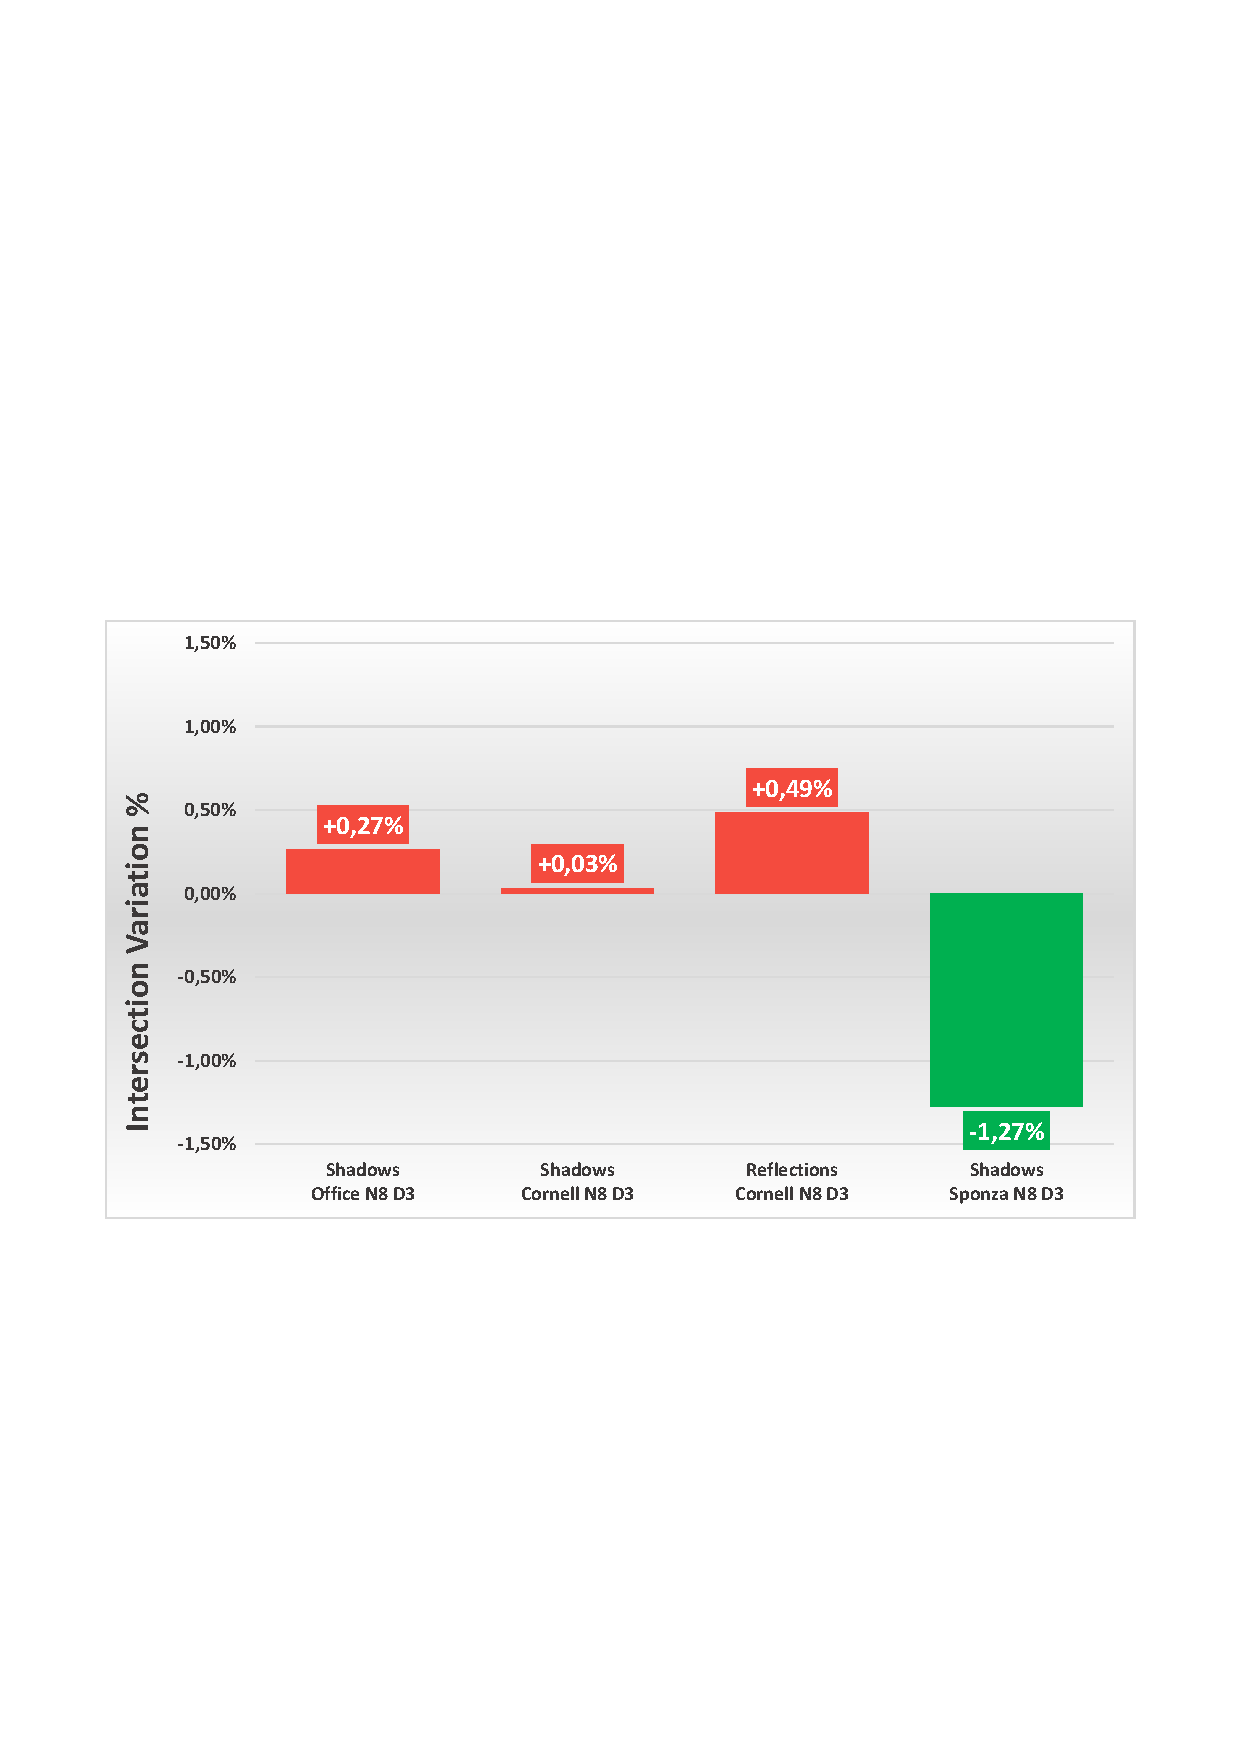
\includegraphics[width=0.85\textwidth]{Images/Chart_Comparison_N8_D2_N8_D3}
    \label{fig:comparison-results-d8-n2-d8-n3}
    \caption{Configuration Comparison between Node Subdivision 8 with Hierarchy Depth 2 and Node Subdivision 8 with Hierarchy Depth 3.}
    \end{center}
\end{figure}

For this set of tests we used a node subdivision of 8 and a hierarchy depth of 3. This means that every node in the upper levels of the hierarchy consists of 8 nodes in the level directly below. We compared this configuration with the baseline configuration of node subdivision of 8 and hierarchy depth of 2.

\subsubsection{Office}

Like our previous tests results, this configuration manages to outperform the RAH algorithm once more (see Table~\ref{table:office-d8-n3-results}). We compute 59,18\% less intersections than RAH on this scene and 97,87\% less than a brute force approach. There is however an increase in the number of intersection tests compared to the baseline configuration. The baseline configuration computes 1.86\% of the brute force intersection total while this configuration computes 2.13\%, a difference of 0.27\%, which amounts to about 13\% more intersection tests (see Figure~\ref{fig:comparison-results-d8-n2-d8-n3}).

\subsubsection{Cornell}

For the Cornell scene we compute 24,33\% less intersections overall (shadow and reflection rays combined) than the RAH algorithm and 90,83\% less than the brute force approach (see Table~\ref{table:cornell-d8-n3-results}). Like in the Office scene there is an increase in the intersection total, from 7.45\% to 7.48\% for shadow rays and from 9.46\% to 9.95\% for reflection rays (see Figure~\ref{fig:comparison-results-d8-n2-d8-n3}).

\subsubsection{Sponza}

In the Sponza scene we compute 69,10\% less intersection tests than RAH and 98,89\% than the brute force approach (see Table~\ref{table:sponza-d8-n3-results}). Unlike previous scenes however the number of intersection tests was reduced from 2.38\% to 1.11\% (see Figure~\ref{fig:comparison-results-d8-n2-d8-n3}). This can be explained by the bigger depth of the hierarchy. Since there aren't any object bounding spheres for this scene every single triangle is tested for intersections with the hierarchy's top nodes. This means that most of these triangles are culled at the first step of the traversal, leading to an overall lower number of intersection tests when compared with a hierarchy with lower depth. There should however be a break point after which the increase in depth will yield no further benefits.

%%%%%%%%%%%%%%%%%%%%%%%%%%%%%%%%%%%%%%%%%%%%%%%%%%%%%%%%%%%%%%%%%%%%%%%%%%%%%%%%%%%%%%%%%%%%%%%%%%%%%%%%%%%%%%%%%%%%%%%%%%%%%%%%%%

\pagebreak
\subsection{Hierarchy Traversal Results - Subdivision 8 Depth 4}

\subsubsection{Office}

% Office Discussion

Comparing our algorithm with the RAH algorithm we can see that our algorithm computes 39,18\% less intersections than RAH on this scene. 97,87\% less than a brute force approach (see Table~\ref{table:office-d8-n4-results} and Table~\ref{table:results-d8-n4}).

% Office Table and Figure
    
\begin{figure}[!htb]
    \begin{minipage}{0.25\linewidth}
        \centering
        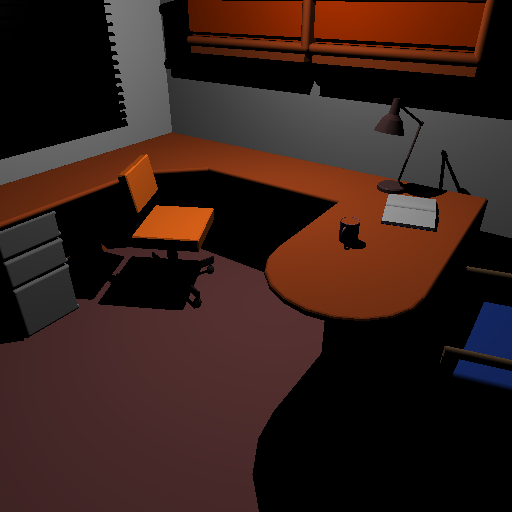
\includegraphics[width=4.0cm]{Images/Office_Preview}
        \captionof{figure}{\textsc{Office}}
    \end{minipage}
    \begin{minipage}{0.725\linewidth}
        \centering
        \fontencoding{T1}
        \fontseries{m}
        \fontshape{sc}
        \fontsize{8}{10}
        \selectfont
        \begin{tabular}[h]{l|rrrr}
            \multicolumn{1}{c|}{\textsc{Office}} & \textsc{Level 4} & \textsc{Level 3} & \textsc{Level 2} & \textsc{Level 1}\\
            \hline
            \emph{RAH Algorithm} & & \\
            \hline
            \quad \# Sh Intersections  & 2251096    & 16736728	& 131228368	& 202025920	\\
            \quad \# Sh Misses         & 159005		& 333182	& 105975128	& 186409563	\\
            \quad \# Sh Hits           & 2092091	& 16403546	& 25253240	& 15616357	\\
            \hline
            \emph{Our Algorithm} & & \\
            \hline
            \quad \# Sh Intersections  & 1398238	& 11068016	& 31896768	& 85725152	\\
            \quad \# Sh Misses         & 14736		& 7080920	& 21181124	& 76679166	\\
            \quad \# Sh Hits           & 1383502	& 3987096	& 10715644	& 9045986	\\
        \end{tabular}
        \label{table:office-d8-n4-results}
        \captionof{table}{\textsc{Office} Division 8 Depth 4 Test Results.}
    \end{minipage}
\end{figure}

\subsubsection{Cornell}

% Cornel Discussion

Comparing our algorithm with the RAH algorithm we can see that our algorithm computes 26,47\% less intersections than RAH on this scene. 91,17\% less than a brute force approach (see Table~\ref{table:cornell-d8-n4-results} and Table~\ref{table:results-d8-n4}).

% Cornell Table and Figure

\begin{figure}[!htb]
    \begin{minipage}{0.25\linewidth}
        \centering
        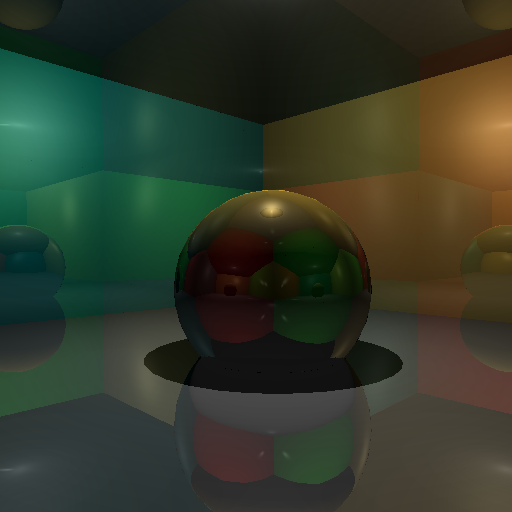
\includegraphics[width=4.0cm]{Images/Cornell_Preview}
        \captionof{figure}{\textsc{Cornell}}
    \end{minipage}
    \begin{minipage}{0.725\linewidth}
        \centering
        \fontencoding{T1}
        \fontseries{m}
        \fontshape{sc}
        \fontsize{8}{10}
        \selectfont
        \begin{tabular}[h]{l|rrrr}
            \multicolumn{1}{c|}{\textsc{Office}} & \textsc{Level 4} & \textsc{Level 3} & \textsc{Level 2} & \textsc{Level 1}\\
            \hline
            \emph{RAH Algorithm} & & \\
            \hline
            \quad \# Sh Intersections   & 47520	    & 335304    & 2617944	& 5150792   \\
            \quad \# Sh Misses          & 5607	    & 8061		& 1974095	& 3600819	\\
            \quad \# Sh Hits            & 41913	    & 327243	& 643849	& 1549973	\\
            & & \\
            \quad \# Re Intersections   & 101376    & 809824	& 6477632   & 17802296  \\
            \quad \# Re Misses          & 148	    & 120	    & 4252345	& 14311812	\\
            \quad \# Re Hits            & 101228	& 809704	& 1284793	& 3490484	\\
            \hline
            \emph{Our Algorithm} & & \\
            \hline
            \quad \# Sh Intersections   & 35280	    & 235248	& 807920	& 2358088	\\
            \quad \# Sh Misses          & 5874		& 134258	& 513159	& 991955	\\
            \quad \# Sh Hits            & 29406	    & 100990    & 294761	& 1366133	\\
            & & \\
            \quad \# Re Intersections   & 101376	& 809808	& 4144632	& 10278344	\\
            \quad \# Re Misses          & 150		& 291729	& 2859839	& 6992777	\\
            \quad \# Re Hits            & 101226	& 518079	& 1284793	& 3285567	\\            
        \end{tabular}
        \label{table:cornell-d8-n4-results}
        \captionof{table}{\textsc{Cornell} Division 8 Depth 4 Test Results.}
    \end{minipage}
\end{figure}

\subsubsection{Sponza}

% Sponza Discussion

Comparing our algorithm with the RAH algorithm we can see that our algorithm computes 35,86\% less intersections than RAH on this scene. 97,62\% less than a brute force approach (see Table~\ref{table:cornell-d8-n4-results} and Table~\ref{table:results-d8-n4}).

% Sponza Table and Figure

\begin{figure}[!htb]
    \begin{minipage}{0.25\linewidth}
        \centering
        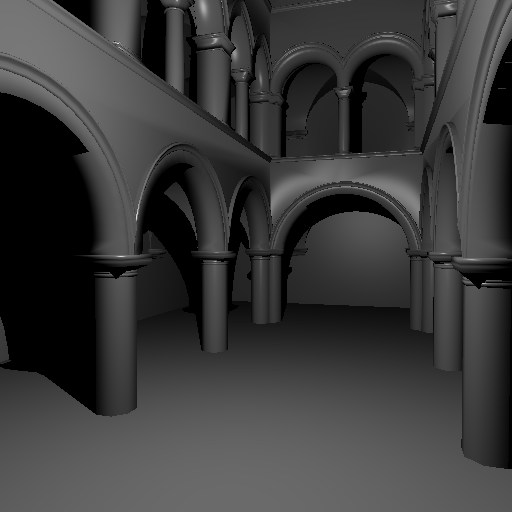
\includegraphics[width=4.0cm]{Images/Sponza_Preview}
        \captionof{figure}{\textsc{Sponza}}
    \end{minipage}
    \begin{minipage}{0.725\linewidth}
        \centering
        \fontencoding{T1}
        \fontseries{m}
        \fontshape{sc}
        \fontsize{8}{10}
        \selectfont
        \begin{tabular}[h]{l|rrrr}
            \multicolumn{1}{c|}{\textsc{Office}} & \textsc{Level 4} & \textsc{Level 3} & \textsc{Level 2} & \textsc{Level 1}\\
            \hline
            \emph{RAH Algorithm} & & \\
            \hline
            \quad \# Sh Intersections   & 4186350	& 27458720  & 214961944	& 261132816	\\
            \quad \# Sh Misses          & 754010	& 588477	& 182320342	& 248455163	\\
            \quad \# Sh Hits            & 3432340	& 26870243	& 32641602	& 12677653	\\
            & & \\
            \hline
            \emph{Our Algorithm} & & \\
            \hline
            \quad \# Sh Intersections   & 4186350	& 12578168	& 23263056	& 61112376	\\
            \quad \# Sh Misses          & 2614079	& 9670286	& 15624009	& 53120871	\\
            \quad \# Sh Hits            & 1572271	& 2907882	& 7639047	& 7991505	\\
        \end{tabular}
        \label{table:sponza-d8-n4-results}
        \captionof{table}{\textsc{Sponza} Division 8 Depth 4 Test Results.}
    \end{minipage}
\end{figure}

\subsection{Hierarchy Traversal Discussion - Subdivision 8 Depth 4}

% Comparison Table

\begin{table}[!htb]
    \begin{center}
    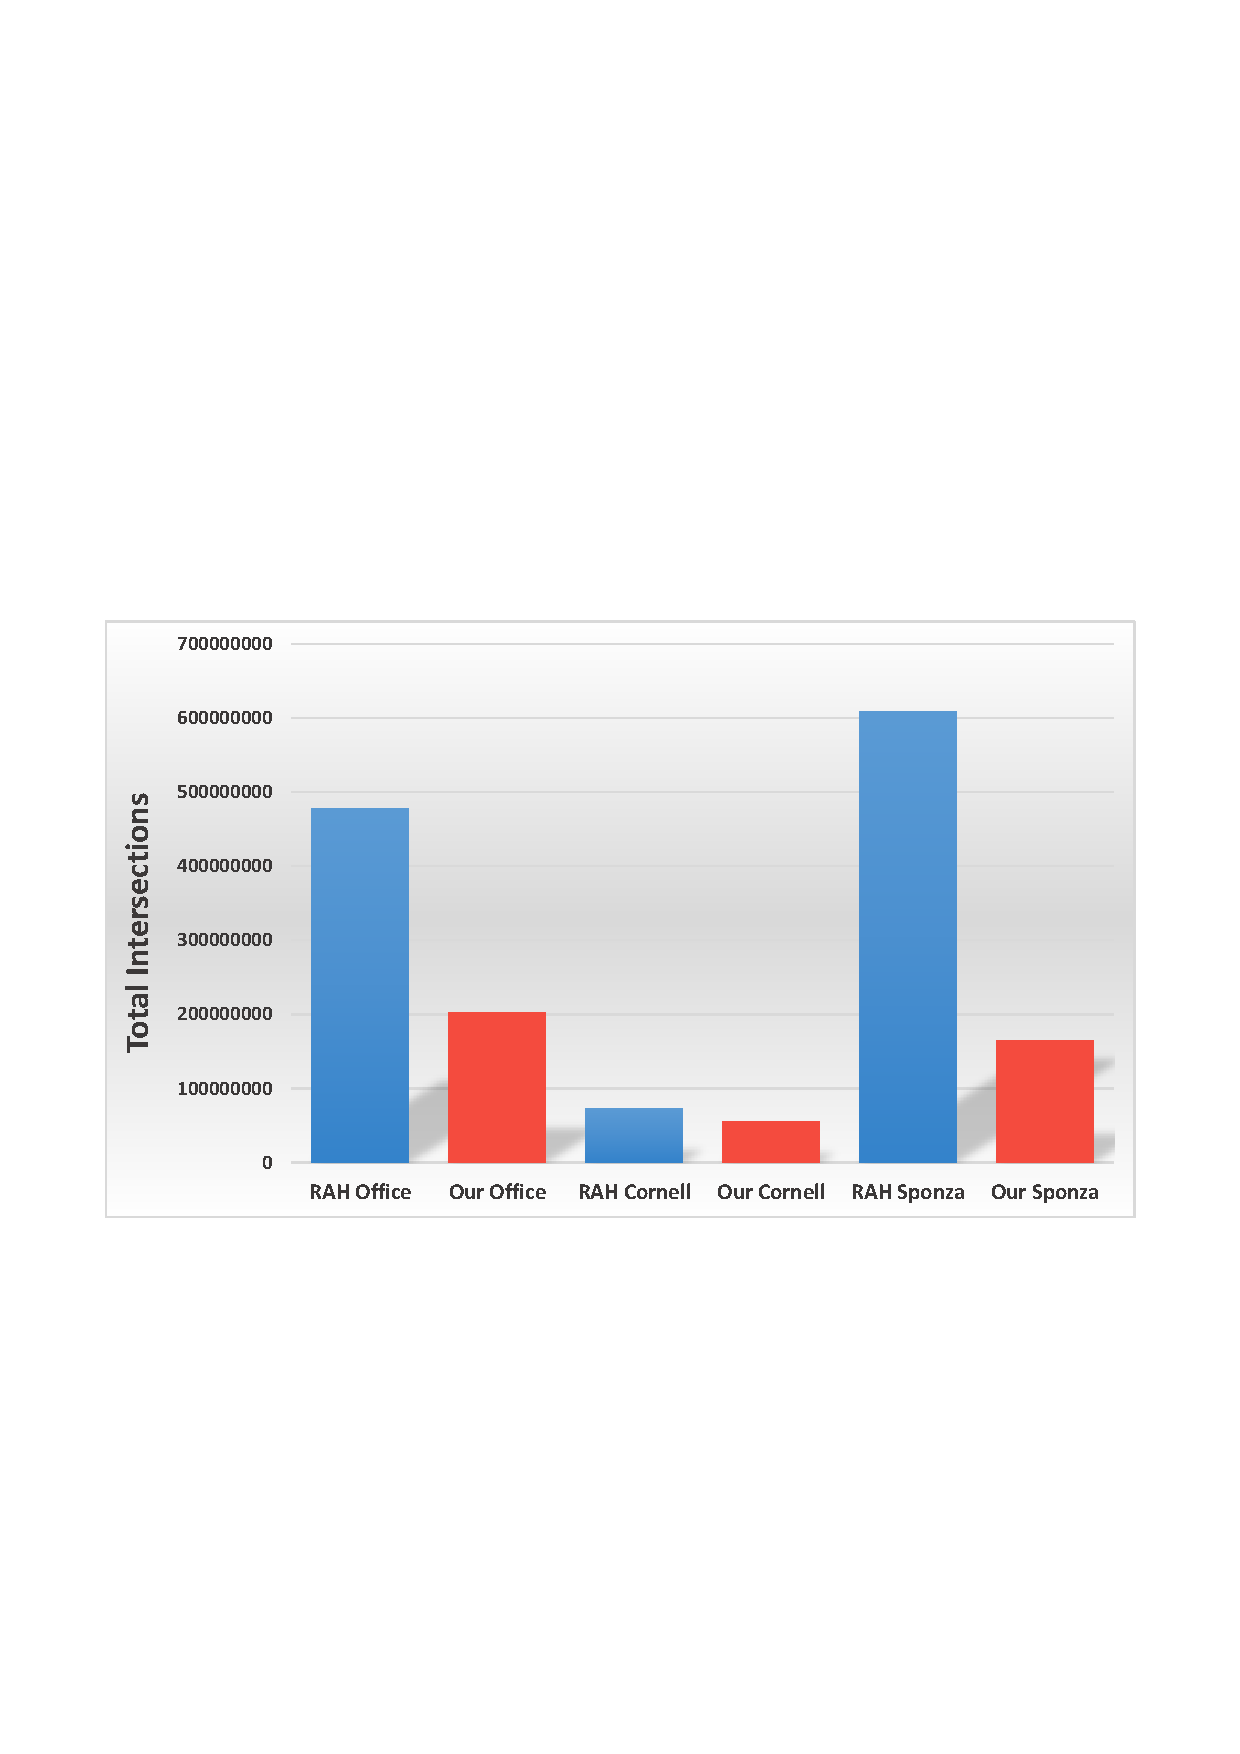
\includegraphics[width=0.85\textwidth]{Images/Chart_N8_D4}
    \vskip 2em
    \fontencoding{T1}
    \fontseries{m}
    \fontshape{sc}
    \fontsize{8}{10}
    \selectfont
    \begin{tabular}{l|rrrrrr}
    & \multicolumn{2}{c}{\textsc{Office}} & \multicolumn{2}{c}{\textsc{Cornell}} & \multicolumn{2}{c}{\textsc{Sponza}} \\
    \textsc{Algorithm} & \textsc{Total \# isect} & \textsc{Relative \%} & \textsc{Total \# isect} & \textsc{Relative \%} & \textsc{Total \# isect} & \textsc{Relative \%} \\
        \hline
        \emph{Brute Force}     & 9133132168         & 100\%           & 606911976         & 100\%           & 17058578850        & 100\% \\
        \emph{RAH Algorithm}   & 477172968			& 5.22\%          & 73666344		  & 12.14\%         & 609161054			 & 3.57\% \\
        \emph{Our Algorithm}   & \textbf{202456062} & \textbf{2.22\%} & \textbf{55984296} & \textbf{9.22\%} & \textbf{165071990} & \textbf{0.97\%} \\
    \end{tabular}
    \end{center}
    \caption{\label{table:results-d8-n4}
    \small\textsc{Office} (251546 shadow rays), \textsc{Cornell} (242015 shadow \& 524288 reflection rays), \textsc{Sponza} (256713 shadow rays) rendering performance using node subdivision 8 and hierarchy depth 4.}
\end{table}

\begin{figure}[!htb]
    \begin{center}
    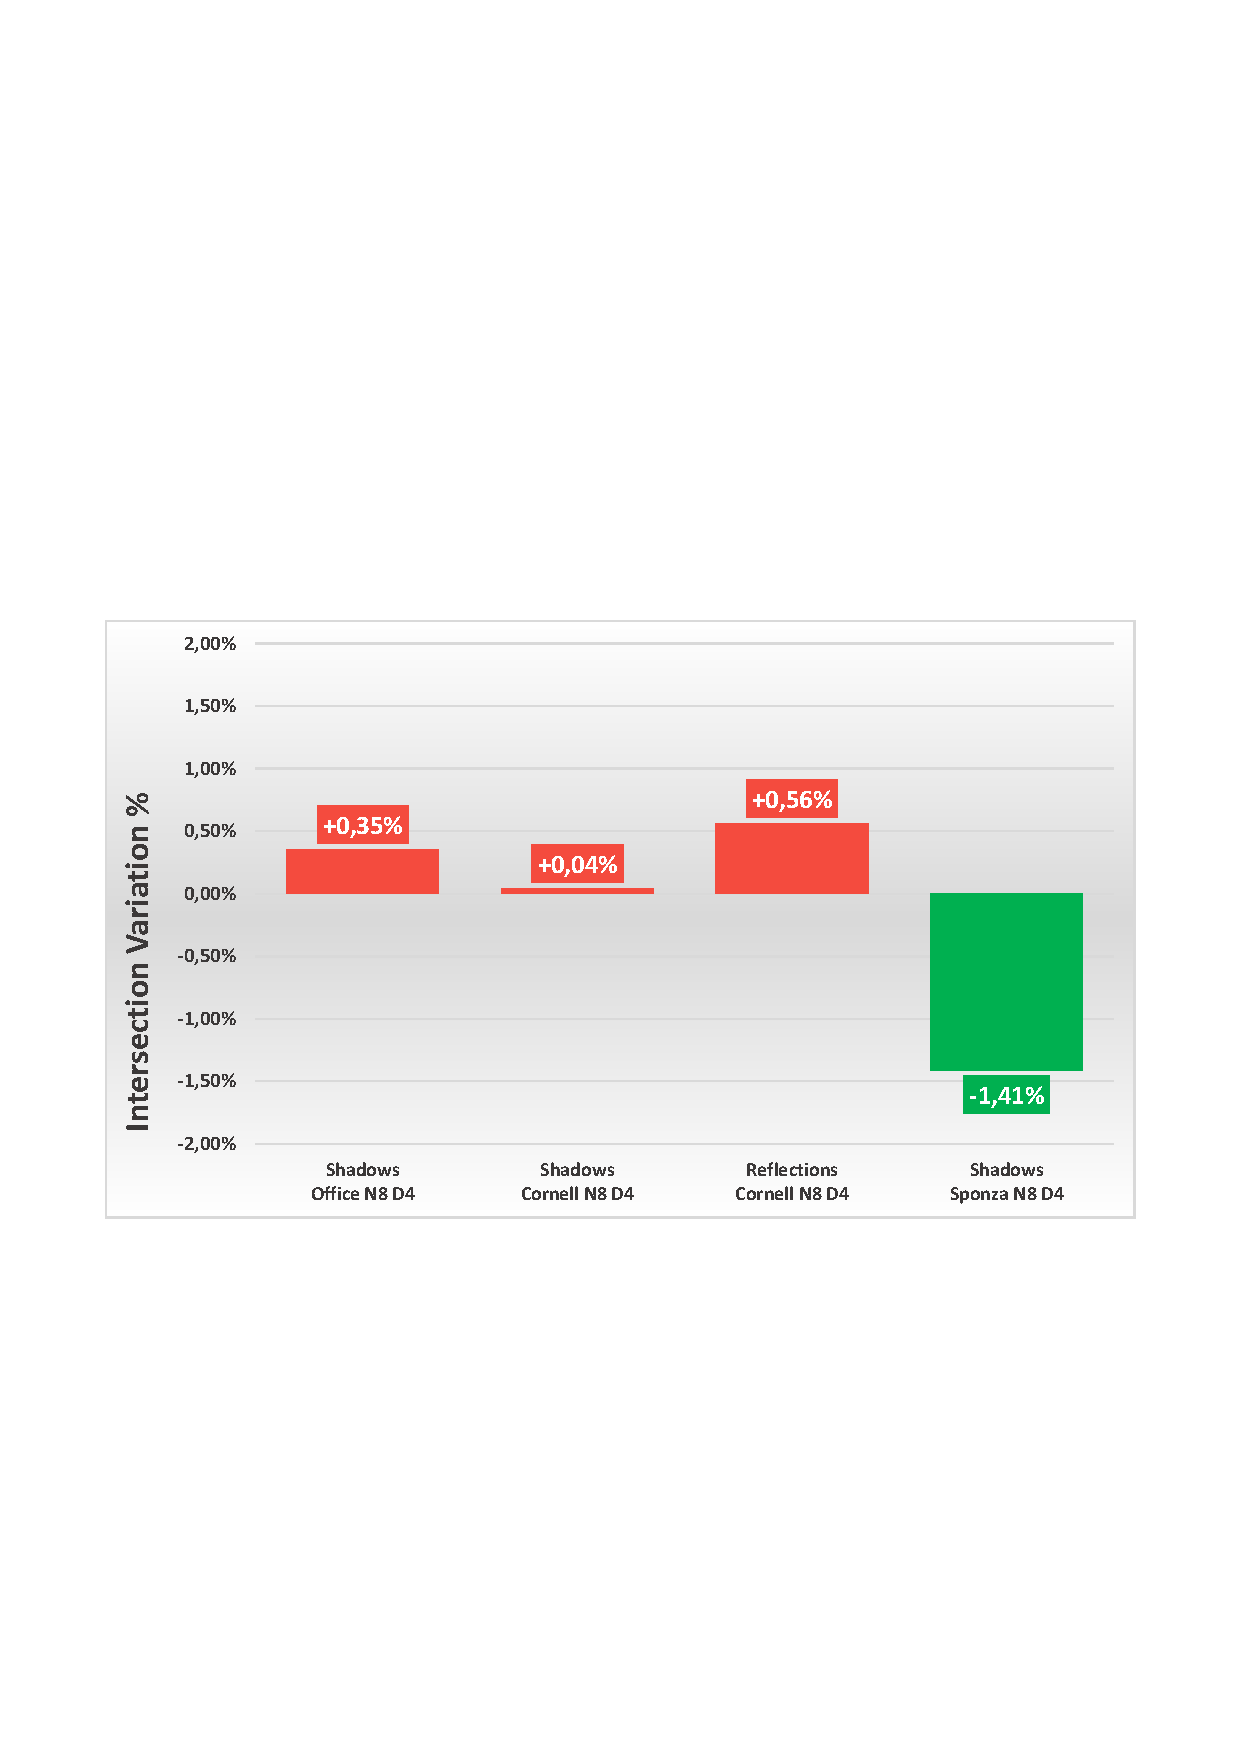
\includegraphics[width=0.70\textwidth]{Images/Chart_Comparison_N8_D2_N8_D4}
    \label{fig:comparison-results-d8-n2-d8-n4}
    \caption{Configuration Comparison between Node Subdivision 8 with Hierarchy Depth 2 and Node Subdivision 8 with Hierarchy Depth 4.}
    \end{center}
\end{figure}

For this set of tests we used a node subdivision of 8 and a hierarchy depth of 4. This means that every node in the upper levels of the hierarchy consists of 8 nodes in the level directly below. We compared this configuration with the baseline configuration of node subdivision of 8 and hierarchy depth of 2.

\subsubsection{Office}

Like our previous tests results, this configuration manages to outperform the RAH algorithm once more (see Table~\ref{table:office-d8-n4-results}). We compute 57,57\% less intersections than RAH on this scene and 97,78\% less than a brute force approach. The tendency for an increase in the intersection total shown in the previous comparison continued for this test. There is an increase from 1.86\% to 2,22\% of the brute force intersection total (see Figure~\ref{fig:comparison-results-d8-n2-d8-n4}).

\subsubsection{Cornell}

For the Cornell scene we compute 24,00\% less intersections overall (shadow and reflection rays combined) than the RAH algorithm and 90,78\% less than the brute force approach (see Table~\ref{table:cornell-d8-n4-results}). Like in the Office scene the tendency for an increase in the intersection total remains as we increase the hierarchies depth. The percentage rose from 7.45\% to 7.49\% for shadow rays and from 9.46\% to 10.02\% for reflection rays (see Figure~\ref{fig:comparison-results-d8-n2-d8-n4}).

\subsubsection{Sponza}

In the Sponza scene we compute 72,90\% less intersection tests than RAH and 99,03\% than the brute force approach (see Table~\ref{table:sponza-d8-n4-results}). The number of intersection tests was reduced once again, going from 2.38\% to 0.97\% (see Figure~\ref{fig:comparison-results-d8-n2-d8-n4}). Our hypothesis remains consistent since as we increase the hierarchy's depth the number of overall intersections keeps dropping for this particular scene.

%%%%%%%%%%%%%%%%%%%%%%%%%%%%%%%%%%%%%%%%%%%%%%%%%%%%%%%%%%%%%%%%%%%%%%%%%%%%%%%%%%%%%%%%%%%%%%%%%%%%%%%%%%%%%%%%%%%%%%%%%%%%%%%%%%

\pagebreak
\subsection{Hierarchy Traversal Results - Subdivision 16 Depth 2}

\subsubsection{Office}

% Office Discussion

Comparing our algorithm with the RAH algorithm we can see that our algorithm computes 39,18\% less intersections than RAH on this scene. 97,87\% less than a brute force approach (see Table~\ref{table:office-d16-n2-results} and Table~\ref{table:results-d16-n2}).

% Office Table and Figure
    
\begin{figure}[!htb]
    \begin{minipage}{0.25\linewidth}
        \centering
        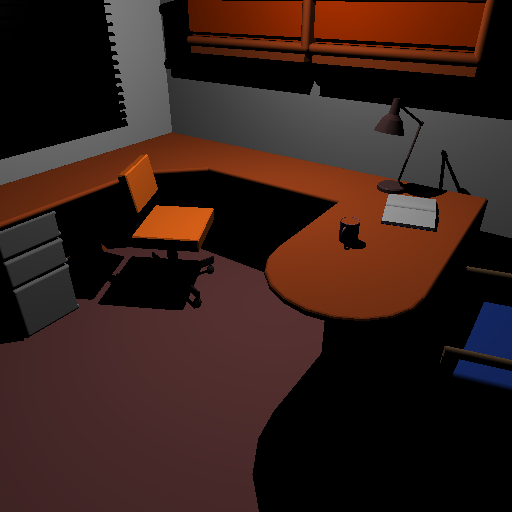
\includegraphics[width=4.0cm]{Images/Office_Preview}
        \captionof{figure}{\textsc{Office}}
    \end{minipage}
    \begin{minipage}{0.725\linewidth}
        \centering
        \fontencoding{T1}
        \fontseries{m}
        \fontshape{sc}
        \fontsize{8}{10}
        \selectfont
        \begin{tabular}[h]{l|rr}
            \multicolumn{1}{c|}{\textsc{Office}} & \textsc{Level 2} & \textsc{Level 1}\\
            \hline
            \emph{RAH Algorithm} & & \\
            \hline
            \quad \# Sh Intersections   & 35690764	& 412453440	\\
            \quad \# Sh Misses          & 9912424	& 398662535	\\
            \quad \# Sh Hits            & 25778340  & 13790905	\\
            \hline
            \emph{Our Algorithm} & & \\
            \hline
            \quad \# Sh Intersections  & 7724430    & 119385600	\\
            \quad \# Sh Misses         & 262830	    & 112687674	\\
            \quad \# Sh Hits           & 7461600	& 6697926	\\
        \end{tabular}
        \label{table:office-d16-n2-results}
        \captionof{table}{\textsc{Office} Division 16 Depth 2 Test Results.}
    \end{minipage}
\end{figure}

\subsubsection{Cornell}

% Cornel Discussion

Comparing our algorithm with the RAH algorithm we can see that our algorithm computes 26,47\% less intersections than RAH on this scene. 91,17\% less than a brute force approach (see Table~\ref{table:cornell-d16-n2-results} and Table~\ref{table:results-d16-n2}).

% Cornell Table and Figure

\begin{figure}[!htb]
    \begin{minipage}{0.25\linewidth}
        \centering
        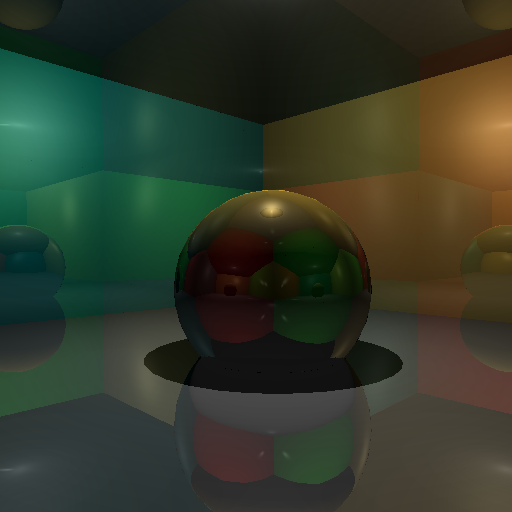
\includegraphics[width=4.0cm]{Images/Cornell_Preview}
        \captionof{figure}{\textsc{Cornell}}
    \end{minipage}
    \begin{minipage}{0.725\linewidth}
        \centering
        \fontencoding{T1}
        \fontseries{m}
        \fontshape{sc}
        \fontsize{8}{10}
        \selectfont
        \begin{tabular}[h]{l|rr}
            \multicolumn{1}{c|}{\textsc{Office}} & \textsc{Level 2} & \textsc{Level 1}\\
            \hline
            \emph{RAH Algorithm} & & \\
            \hline
            \quad \# Sh Intersections   & 749232    & 7732000	\\
            \quad \# Sh Misses          & 265982	& 6808346	\\
            \quad \# Sh Hits            & 483250	& 923654	\\
            & & \\
            \quad \# Re Intersections   & 1622016	& 23053680	\\
            \quad \# Re Misses          & 181161	& 20614507  \\
            \quad \# Re Hits            & 1440855	& 2439173   \\
            \hline
            \emph{Our Algorithm} & & \\
            \hline
            \quad \# Sh Intersections   & 343872    & 2571952	\\
            \quad \# Sh Misses          & 183125	& 1846363	\\
            \quad \# Sh Hits            & 160747	& 725589	\\
            & & \\
            \quad \# Re Intersections   & 983928	& 11460592	\\
            \quad \# Re Misses          & 267641	& 9368514	\\
            \quad \# Re Hits            & 716287	& 2092078	\\            
        \end{tabular}
        \label{table:cornell-d16-n2-results}
        \captionof{table}{\textsc{Cornell} Division 16 Depth 2 Test Results.}
    \end{minipage}
\end{figure}

\subsubsection{Sponza}

% Sponza Discussion

Comparing our algorithm with the RAH algorithm we can see that our algorithm computes 35,86\% less intersections than RAH on this scene. 97,62\% less than a brute force approach (see Table~\ref{table:sponza-d16-n2-results} and Table~\ref{table:results-d16-n2}).

% Sponza Table and Figure

\begin{figure}[!htb]
    \begin{minipage}{0.25\linewidth}
        \centering
        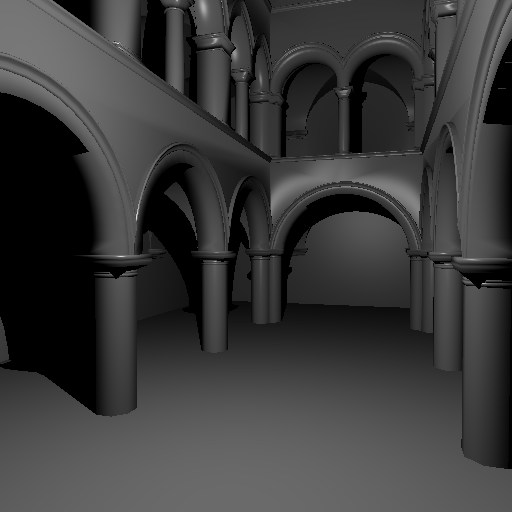
\includegraphics[width=4.0cm]{Images/Sponza_Preview}
        \captionof{figure}{\textsc{Sponza}}
    \end{minipage}
    \begin{minipage}{0.725\linewidth}
        \centering
        \fontencoding{T1}
        \fontseries{m}
        \fontshape{sc}
        \fontsize{8}{10}
        \selectfont
        \begin{tabular}[h]{l|rr}
            \multicolumn{1}{c|}{\textsc{Office}} & \textsc{Level 2} & \textsc{Level 1}\\
            \hline
            \emph{RAH Algorithm} & & \\
            \hline
            \quad \# Sh Intersections   & 66649350	& 554494192	\\
            \quad \# Sh Misses          & 31993463	& 544455870	\\
            \quad \# Sh Hits            & 34655887	& 10038322	\\
            & & \\
            \hline
            \emph{Our Algorithm} & & \\
            \hline
            \quad \# Sh Intersections   & 66649350	& 103145120	\\
            \quad \# Sh Misses          & 60202780	& 97483134	\\
            \quad \# Sh Hits            & 6446570	& 5661986	\\
        \end{tabular}
        \label{table:sponza-d16-n2-results}
        \captionof{table}{\textsc{Sponza} Division 16 Depth 2 Test Results.}
    \end{minipage}
\end{figure}

\subsection{Hierarchy Traversal Discussion - Subdivision 16 Depth 2}

% Comparison Table

\begin{table}[!htb]
    \begin{center}
    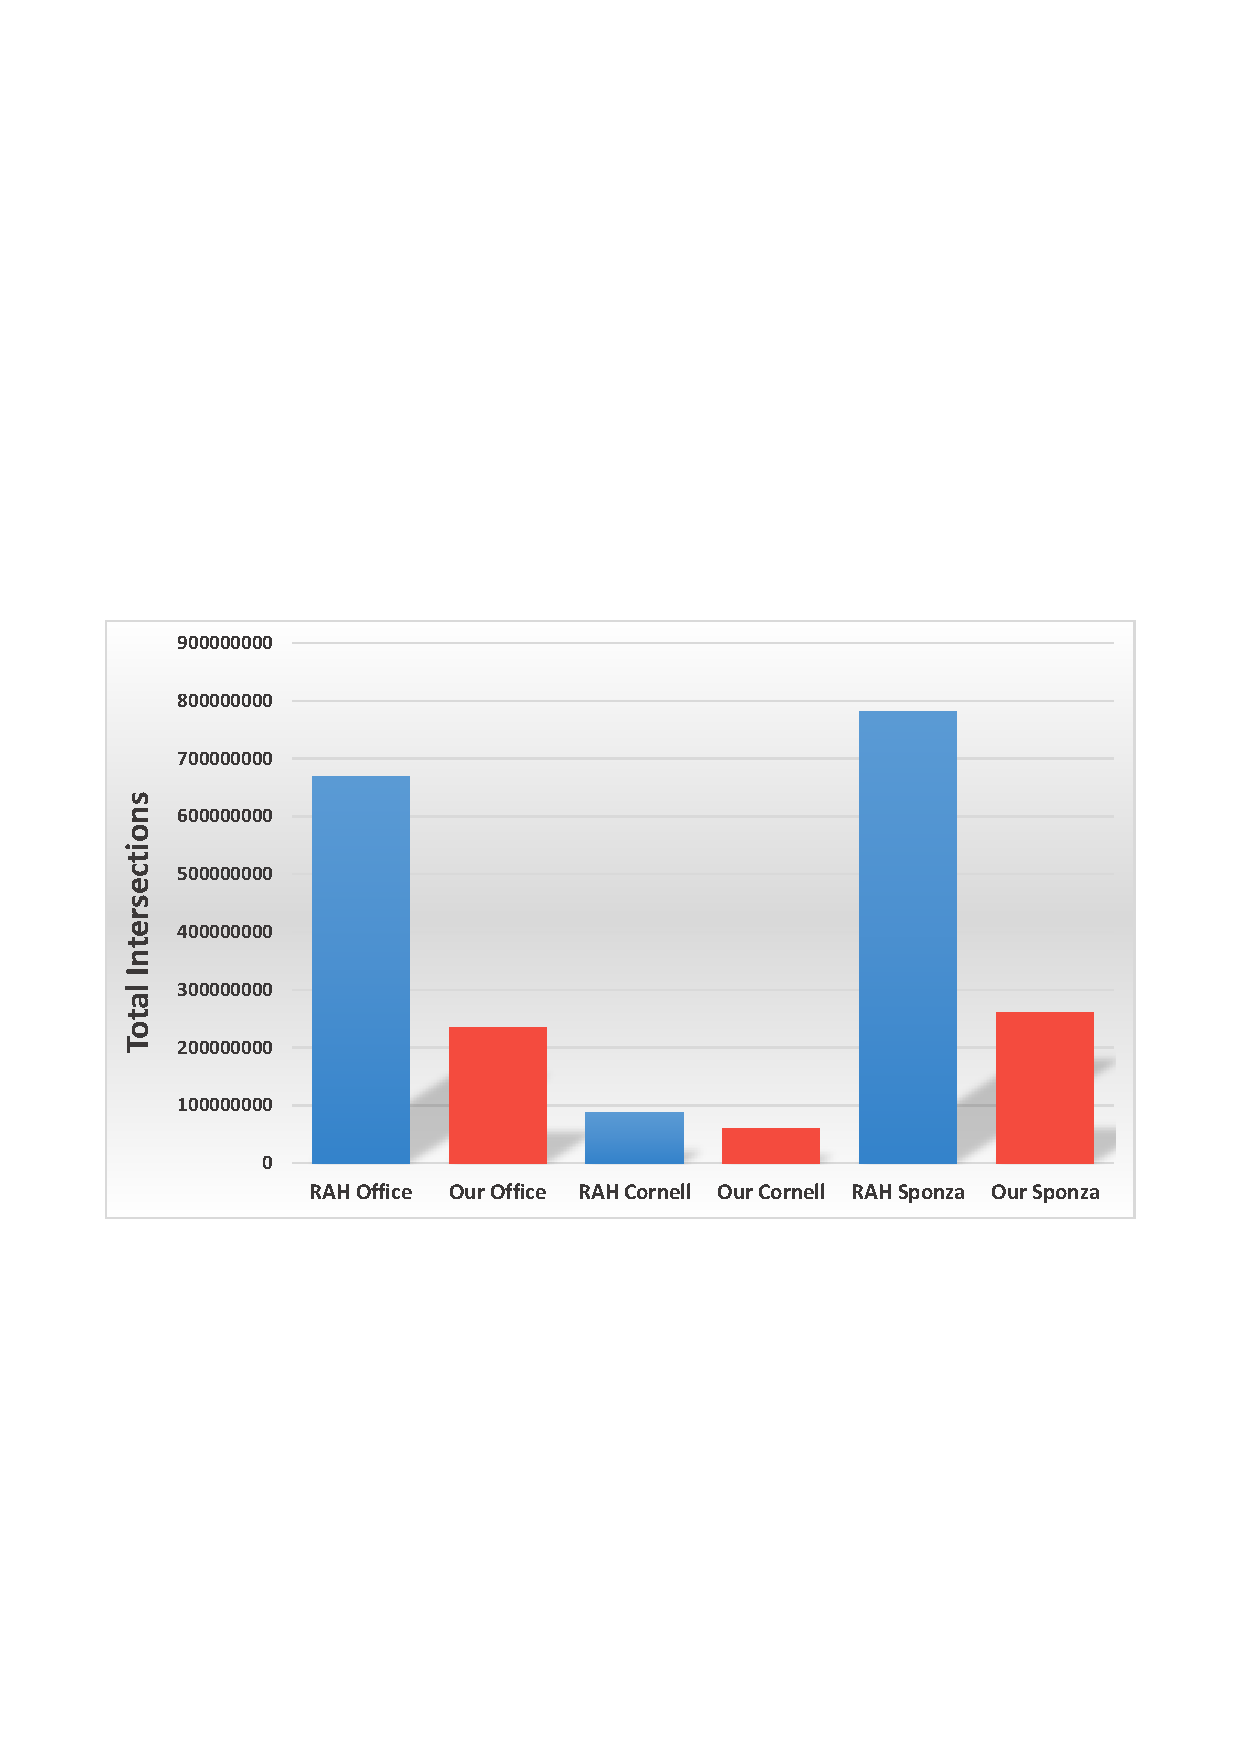
\includegraphics[width=0.85\textwidth]{Images/Chart_N16_D2}
    \vskip 2em
    \fontencoding{T1}
    \fontseries{m}
    \fontshape{sc}
    \fontsize{8}{10}
    \selectfont
    \begin{tabular}{l|rrrrrr}
    & \multicolumn{2}{c}{\textsc{Office}} & \multicolumn{2}{c}{\textsc{Cornell}} & \multicolumn{2}{c}{\textsc{Sponza}} \\
    \textsc{Algorithm} & \textsc{Total \# isect} & \textsc{Relative \%} & \textsc{Total \# isect} & \textsc{Relative \%} & \textsc{Total \# isect} & \textsc{Relative \%} \\
        \hline
        \emph{Brute Force}     & 9133132168         & 100\%           & 606911976           & 100\%           & 17058578850         & 100\% \\
        \emph{RAH Algorithm}   & 668798684		    & 7.32\%          & 86962160            & 14.33\%         & 781756694	        & 4.58\% \\
        \emph{Our Algorithm}   & \textbf{234276846} & \textbf{2.57\%} & \textbf{60443016}	& \textbf{9.96\%} & \textbf{260386246}  & \textbf{1.53\%} \\
    \end{tabular}
    \end{center}
    \caption{\label{table:results-d16-n2}
    \small\textsc{Office} (251546 shadow rays), \textsc{Cornell} (242015 shadow \& 524288 reflection rays), \textsc{Sponza} (256713 shadow rays) rendering performance using node subdivision 16 and hierarchy depth 2.}
\end{table}

\begin{figure}[!htb]
    \begin{center}
    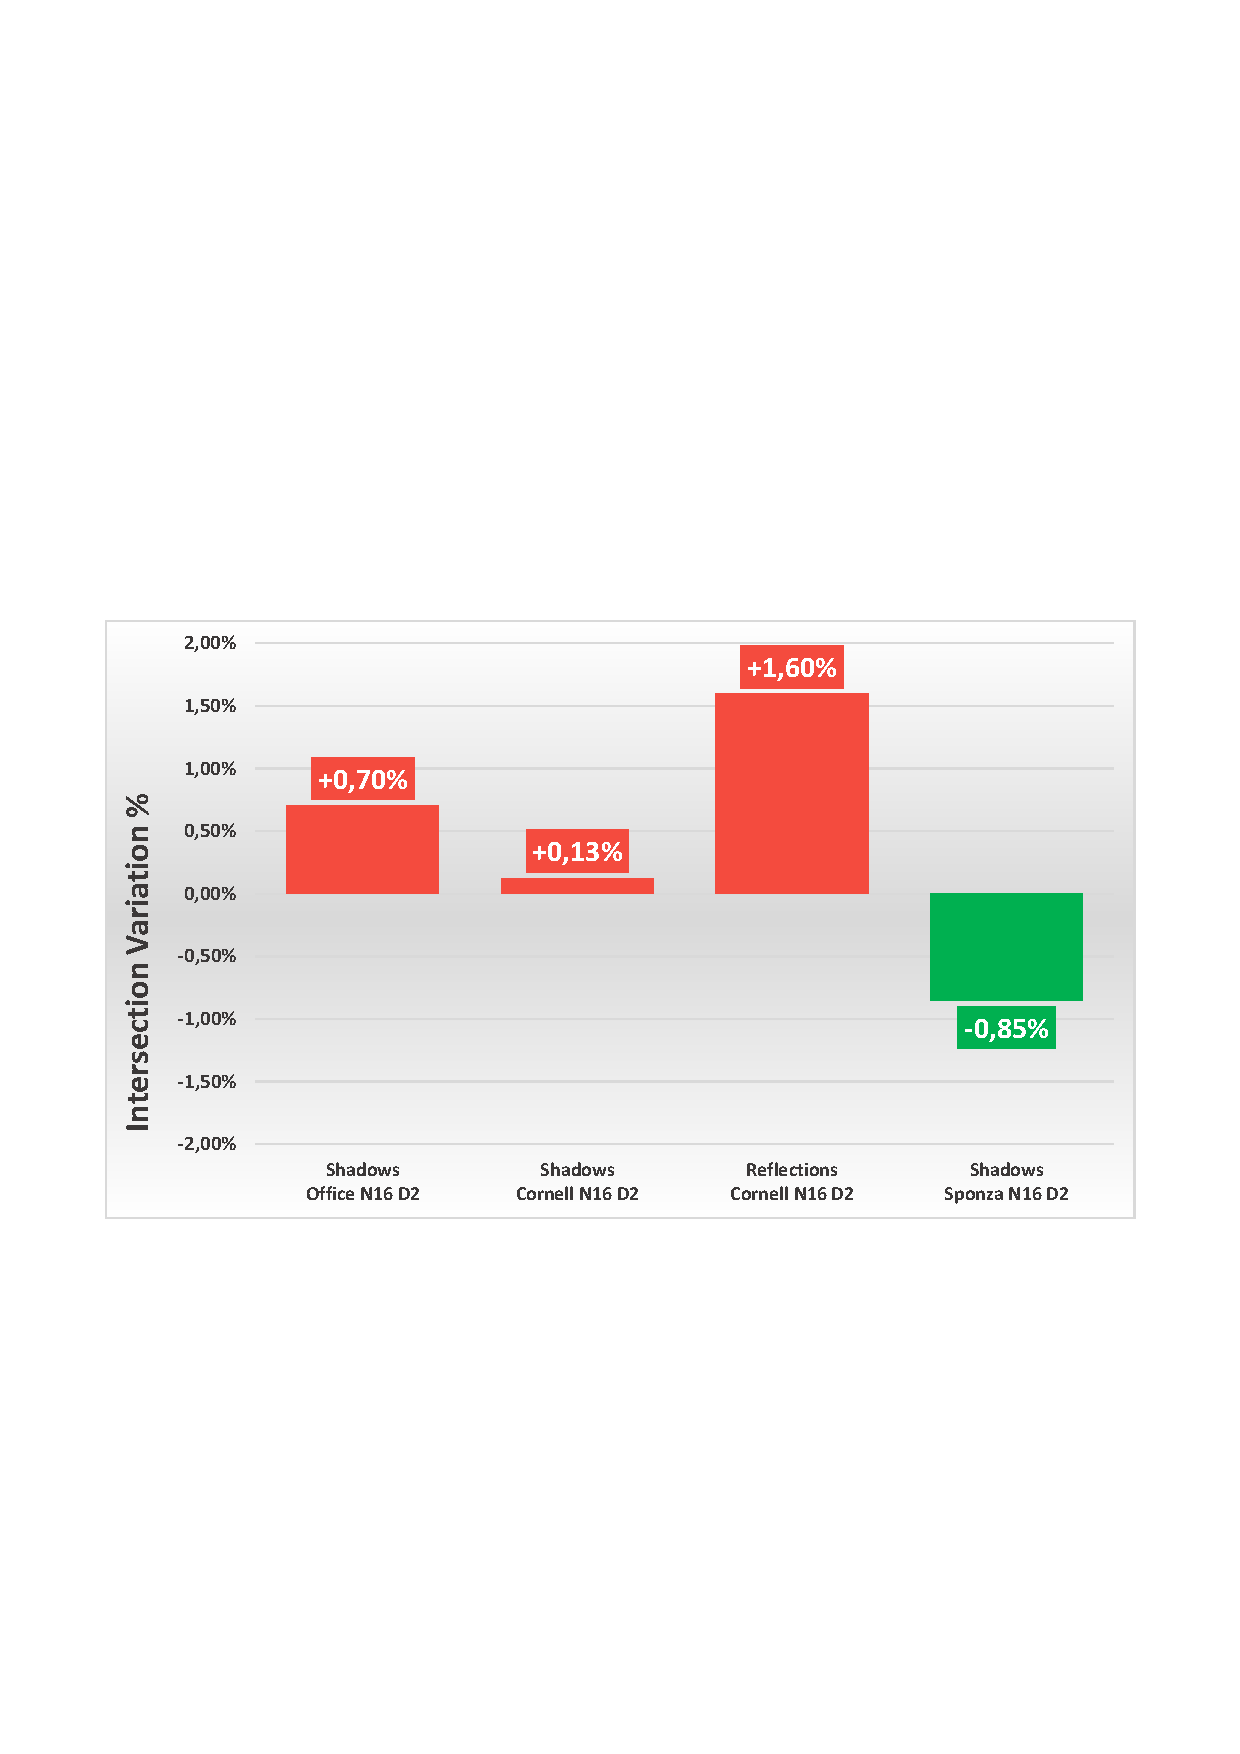
\includegraphics[width=0.70\textwidth]{Images/Chart_Comparison_N8_D2_N16_D2}
    \label{fig:comparison-results-d8-n2-d16-n2}
    \caption{Configuration Comparison between Node Subdivision 8 with Hierarchy Depth 2 and Node Subdivision 16 with Hierarchy Depth 2.}
    \end{center}
\end{figure}

For this set of tests we used a node subdivision of 16 and a hierarchy depth of 2. This means that every node in the upper levels of the hierarchy consists of 16 nodes in the level directly below. We compared this configuration with the baseline configuration of node subdivision of 8 and hierarchy depth of 2.

\subsubsection{Office}

With the new node subdivision this configuration still outperforms the RAH algorithm (see Table~\ref{table:office-d16-n2-results}). We compute 64,97\% less intersections than RAH on this scene and 97,43\% less than a brute force approach. These results are extremely close to the baseline configuration but there is still an increase of 0.70\% when compared to the baseline (from 1.86\% to 2.57\%) (see Figure~\ref{fig:comparison-results-d8-n2-d16-n2}).

\subsubsection{Cornell}

For the Cornell scene we compute 30,50\% less intersections overall (shadow and reflection rays combined) than the RAH algorithm and 90,04\% less than the brute force approach (see Table~\ref{table:cornell-d16-n2-results}). When we compare these results with the baseline configuration we get an increase of 0.13\%, from 7.45\% to 7.58\% for shadow rays and from 9.46\% to 11.06\% for reflection rays (see Figure~\ref{fig:comparison-results-d8-n2-d16-n2}).

\subsubsection{Sponza}

In the Sponza scene we compute 66,69\% less intersection tests than RAH and 98,47\% than the brute force approach (see Table~\ref{table:sponza-d16-n2-results}). The number of intersection tests was reduced once again, going from the baseline 2.38\% to 1.53\% (see Figure~\ref{fig:comparison-results-d8-n2-d16-n2}). This is slightly different from the previous cases but the explanation is very similar. Because every node consists of more rays the upper levels of the hierarchy discard even more test results for the traversal of the lower levels of the hierarchy, leading to the overall reduction in intersections.

%%%%%%%%%%%%%%%%%%%%%%%%%%%%%%%%%%%%%%%%%%%%%%%%%%%%%%%%%%%%%%%%%%%%%%%%%%%%%%%%%%%%%%%%%%%%%%%%%%%%%%%%%%%%%%%%%%%%%%%%%%%%%%%%%%

\pagebreak
\subsection{Hierarchy Traversal Results - Subdivision 16 Depth 3}

\subsubsection{Office}

% Office Discussion

Comparing our algorithm with the RAH algorithm we can see that our algorithm computes 39,18\% less intersections than RAH on this scene. 97,87\% less than a brute force approach (see Table~\ref{table:office-d16-n3-results} and Table~\ref{table:results-d16-n3}).

% Office Table and Figure
    
\begin{figure}[!htb]
    \begin{minipage}{0.25\linewidth}
        \centering
        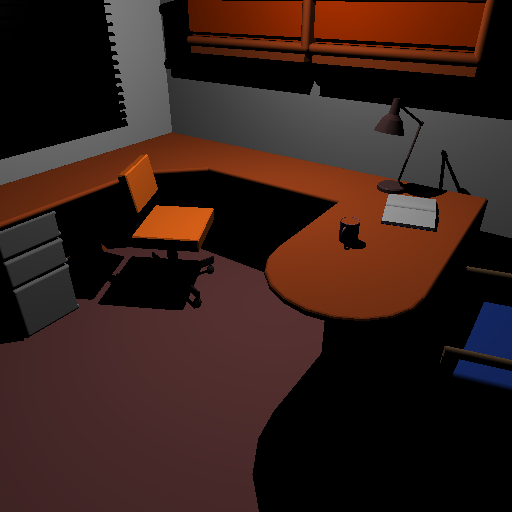
\includegraphics[width=4.0cm]{Images/Office_Preview}
        \captionof{figure}{\textsc{Office}}
    \end{minipage}
    \begin{minipage}{0.725\linewidth}
        \centering
        \fontencoding{T1}
        \fontseries{m}
        \fontshape{sc}
        \fontsize{8}{10}
        \selectfont
        \begin{tabular}[h]{l|rrr}
            \multicolumn{1}{c|}{\textsc{Office}} & \textsc{Level 3} & \textsc{Level 2} & \textsc{Level 1}\\
            \hline
            \emph{RAH Algorithm} & & \\
            \hline
            \quad \# Sh Intersections   & 2251096   & 36017536	& 412453440	\\
            \quad \# Sh Misses          & 0	        & 10239196	& 398662535	\\
            \quad \# Sh Hits            & 2251096	& 25778340  & 13790905	\\
            \hline
            \emph{Our Algorithm} & & \\
            \hline
            \quad \# Sh Intersections  & 1474802	& 23344000	& 119524928	\\
            \quad \# Sh Misses         & 15802		& 15873692	& 112848037	\\
            \quad \# Sh Hits           & 1459000	& 7470308	& 6676891	\\
        \end{tabular}
        \label{table:office-d16-n3-results}
        \captionof{table}{\textsc{Office} Division 16 Depth 3 Test Results.}
    \end{minipage}
\end{figure}

\subsubsection{Cornell}

% Cornel Discussion

Comparing our algorithm with the RAH algorithm we can see that our algorithm computes 26,47\% less intersections than RAH on this scene. 91,17\% less than a brute force approach (see Table~\ref{table:cornell-d16-n3-results} and Table~\ref{table:results-d16-n3}).

% Cornell Table and Figure

\begin{figure}[!htb]
    \begin{minipage}{0.25\linewidth}
        \centering
        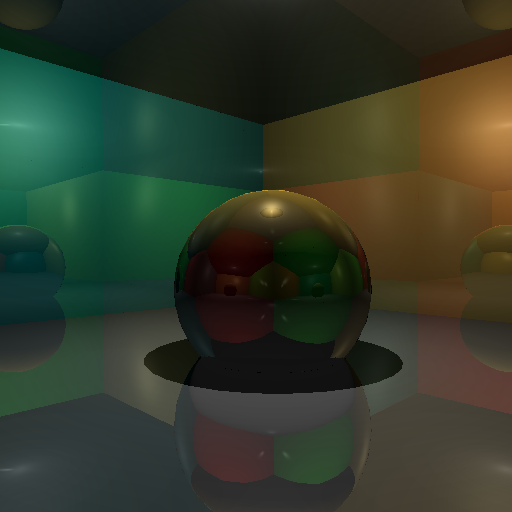
\includegraphics[width=4.0cm]{Images/Cornell_Preview}
        \captionof{figure}{\textsc{Cornell}}
    \end{minipage}
    \begin{minipage}{0.725\linewidth}
        \centering
        \fontencoding{T1}
        \fontseries{m}
        \fontshape{sc}
        \fontsize{8}{10}
        \selectfont
        \begin{tabular}[h]{l|rrr}
            \multicolumn{1}{c|}{\textsc{Office}} & \textsc{Level 3} & \textsc{Level 2} & \textsc{Level 1}\\
            \hline
            \emph{RAH Algorithm} & & \\
            \hline
            \quad \# Sh Intersections       & 47520     & 760128    & 7732000 \\
            \quad \# Sh Misses              & 12		& 276878    & 6808346 \\
            \quad \# Sh Hits                & 47508		& 483250	& 923654  \\
            & & \\
            \quad \# Re Intersections       & 101376	& 1622016	& 23053680  \\
            \quad \# Re Misses              & 0	        & 181161	& 20614507  \\
            \quad \# Re Hits                & 101376	& 1440855	& 2439173	\\
            \hline
            \emph{Our Algorithm} & & \\
            \hline
            \quad \# Sh Intersections       & 36720		& 498352	& 2577680	\\
            \quad \# Sh Misses              & 5573		& 337247	& 1856187	\\
            \quad \# Sh Hits                & 31147		& 161105	& 721493	\\
            & & \\
            \quad \# Re Intersections       & 101376	& 1620432	& 11466336	\\
            \quad \# Re Misses              & 99	    & 903786	& 9374256	\\
            \quad \# Re Hits                & 101277	& 716646	& 2092080	\\            
        \end{tabular}
        \label{table:cornell-d16-n3-results}
        \captionof{table}{\textsc{Cornell} Division 16 Depth 3 Test Results.}
    \end{minipage}
\end{figure}

\subsubsection{Sponza}

% Sponza Discussion

Comparing our algorithm with the RAH algorithm we can see that our algorithm computes 35,86\% less intersections than RAH on this scene. 97,62\% less than a brute force approach (see Table~\ref{table:sponza-d16-n3-results} and Table~\ref{table:results-d16-n3}).

% Sponza Table and Figure

\begin{figure}[!htb]
    \begin{minipage}{0.25\linewidth}
        \centering
        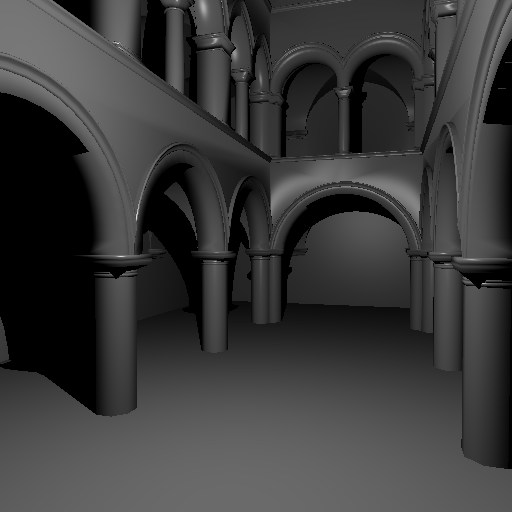
\includegraphics[width=4.0cm]{Images/Sponza_Preview}
        \captionof{figure}{\textsc{Sponza}}
    \end{minipage}
    \begin{minipage}{0.725\linewidth}
        \centering
        \fontencoding{T1}
        \fontseries{m}
        \fontshape{sc}
        \fontsize{8}{10}
        \selectfont
        \begin{tabular}[h]{l|rrr}
            \multicolumn{1}{c|}{\textsc{Office}} & \textsc{Level 3} & \textsc{Level 2} & \textsc{Level 1}\\
            \hline
            \emph{RAH Algorithm} & & \\
            \hline
            \quad \# Sh Intersections   & 4186350   & 66981600	& 554494192	\\
            \quad \# Sh Misses          & 0	        & 32325713	& 544455870	\\
            \quad \# Sh Hits            & 4186350	& 34655887	& 10038322	\\
            & & \\
            \hline
            \emph{Our Algorithm} & & \\
            \hline
            \quad \# Sh Intersections   & 4186350	& 29037376	& 102667568	\\
            \quad \# Sh Misses          & 2371514	& 22620653	& 97483134	\\
            \quad \# Sh Hits            & 1814836	& 6416723	& 5184434	\\
        \end{tabular}
        \label{table:sponza-d16-n3-results}
        \captionof{table}{\textsc{Sponza} Division 16 Depth 3 Test Results.}
    \end{minipage}
\end{figure}

\subsection{Hierarchy Traversal Discussion - Subdivision 16 Depth 3}

% Comparison Table

\begin{table}[!htb]
    \begin{center}
    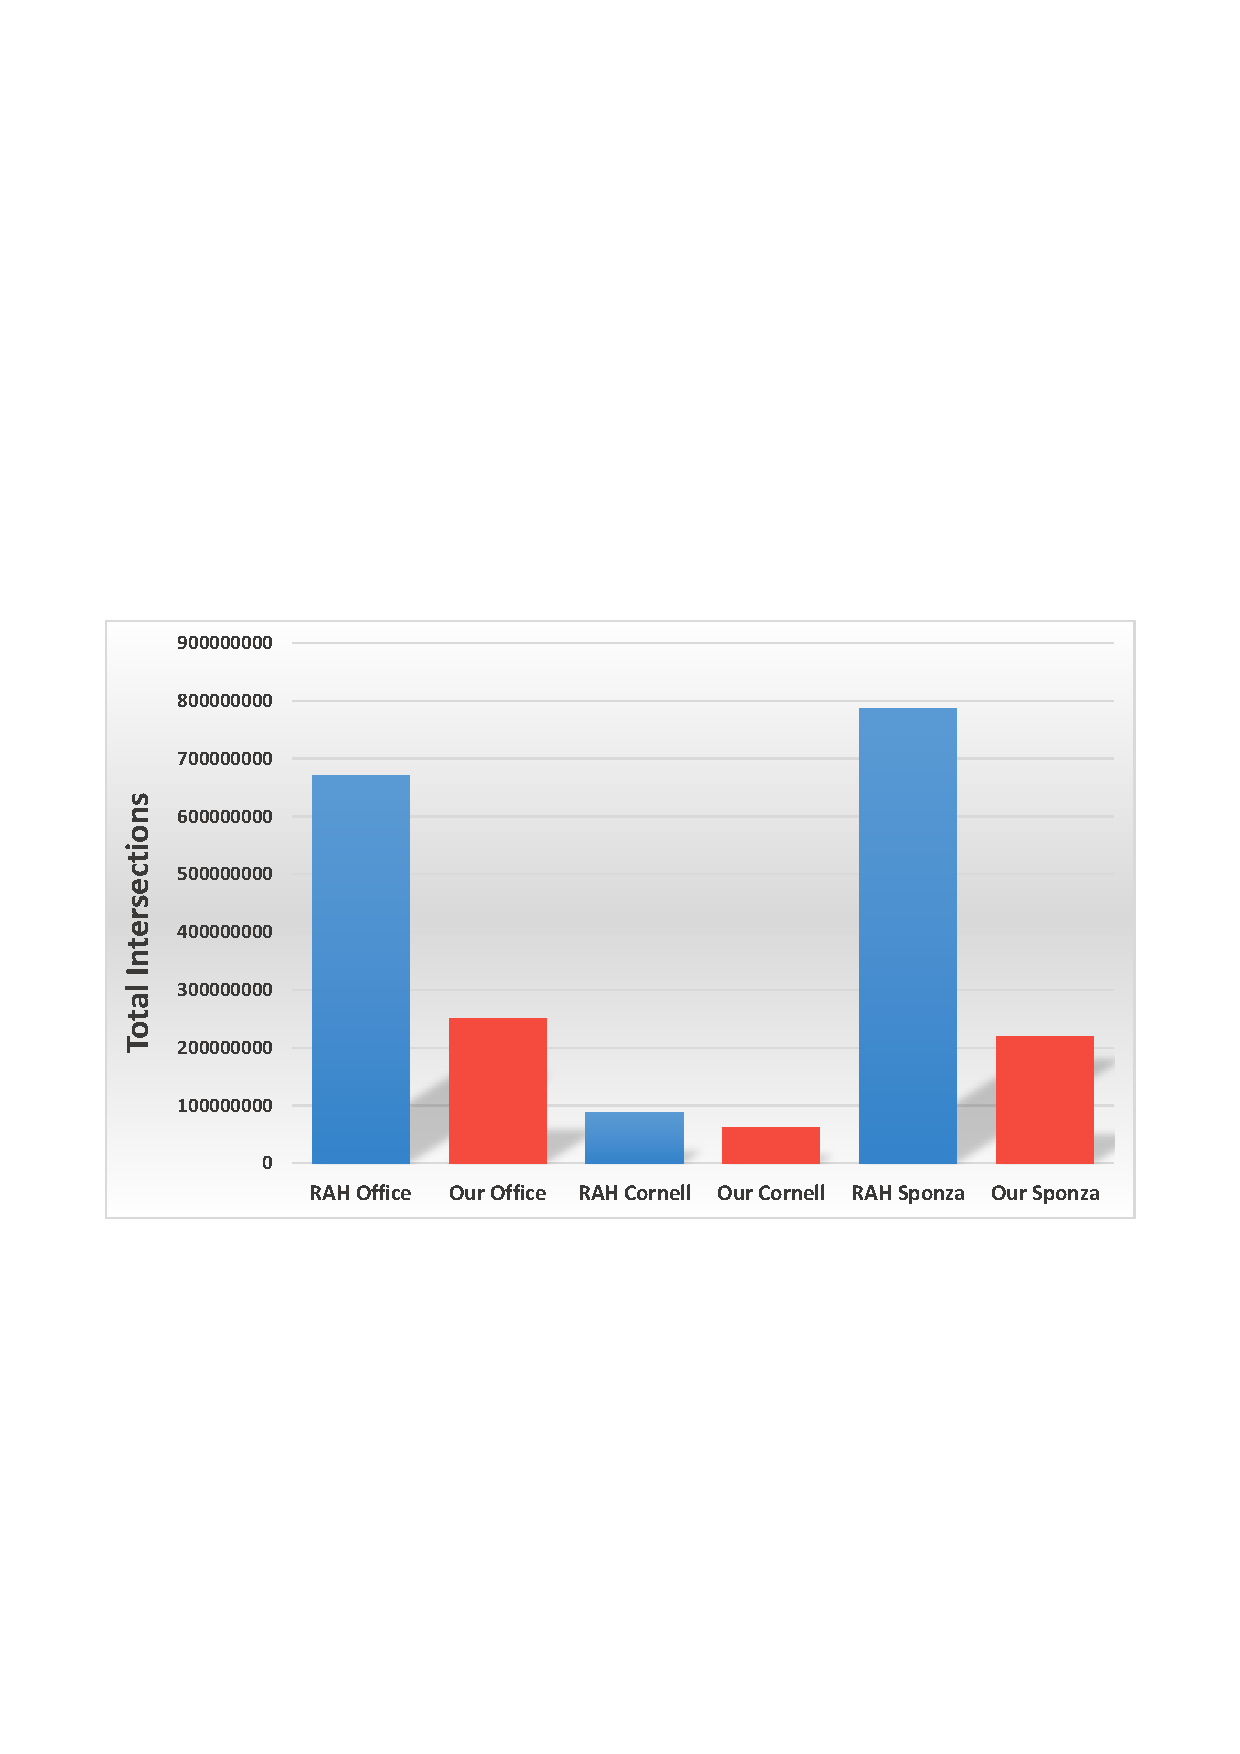
\includegraphics[width=0.85\textwidth]{Images/Chart_N16_D3}
    \vskip 2em
    \fontencoding{T1}
    \fontseries{m}
    \fontshape{sc}
    \fontsize{8}{10}
    \selectfont
    \begin{tabular}{l|rrrrrr}
    & \multicolumn{2}{c}{\textsc{Office}} & \multicolumn{2}{c}{\textsc{Cornell}} & \multicolumn{2}{c}{\textsc{Sponza}} \\
    \textsc{Algorithm} & \textsc{Total \# isect} & \textsc{Relative \%} & \textsc{Total \# isect} & \textsc{Relative \%} & \textsc{Total \# isect} & \textsc{Relative \%} \\
        \hline
        \emph{Brute Force}     & 9133132168         & 100\%           & 606911976         & 100\%           & 17058578850        & 100\% \\
        \emph{RAH Algorithm}   & 671376552			& 7.35\%          & 87121952		  & 14.35\%         & 786275294			 & 4.61\% \\
        \emph{Our Algorithm}   & \textbf{251173986} & \textbf{2.75\%} & \textbf{61318064} & \textbf{10.10\%} & \textbf{218842238} & \textbf{1.28\%} \\
    \end{tabular}
    \end{center}
    \caption{\label{table:results-d16-n3}
    \small\textsc{Office} (251546 shadow rays), \textsc{Cornell} (242015 shadow \& 524288 reflection rays), \textsc{Sponza} (256713 shadow rays) rendering performance using node subdivision 16 and hierarchy depth 3.}
\end{table}

\begin{figure}[!htb]
    \begin{center}
    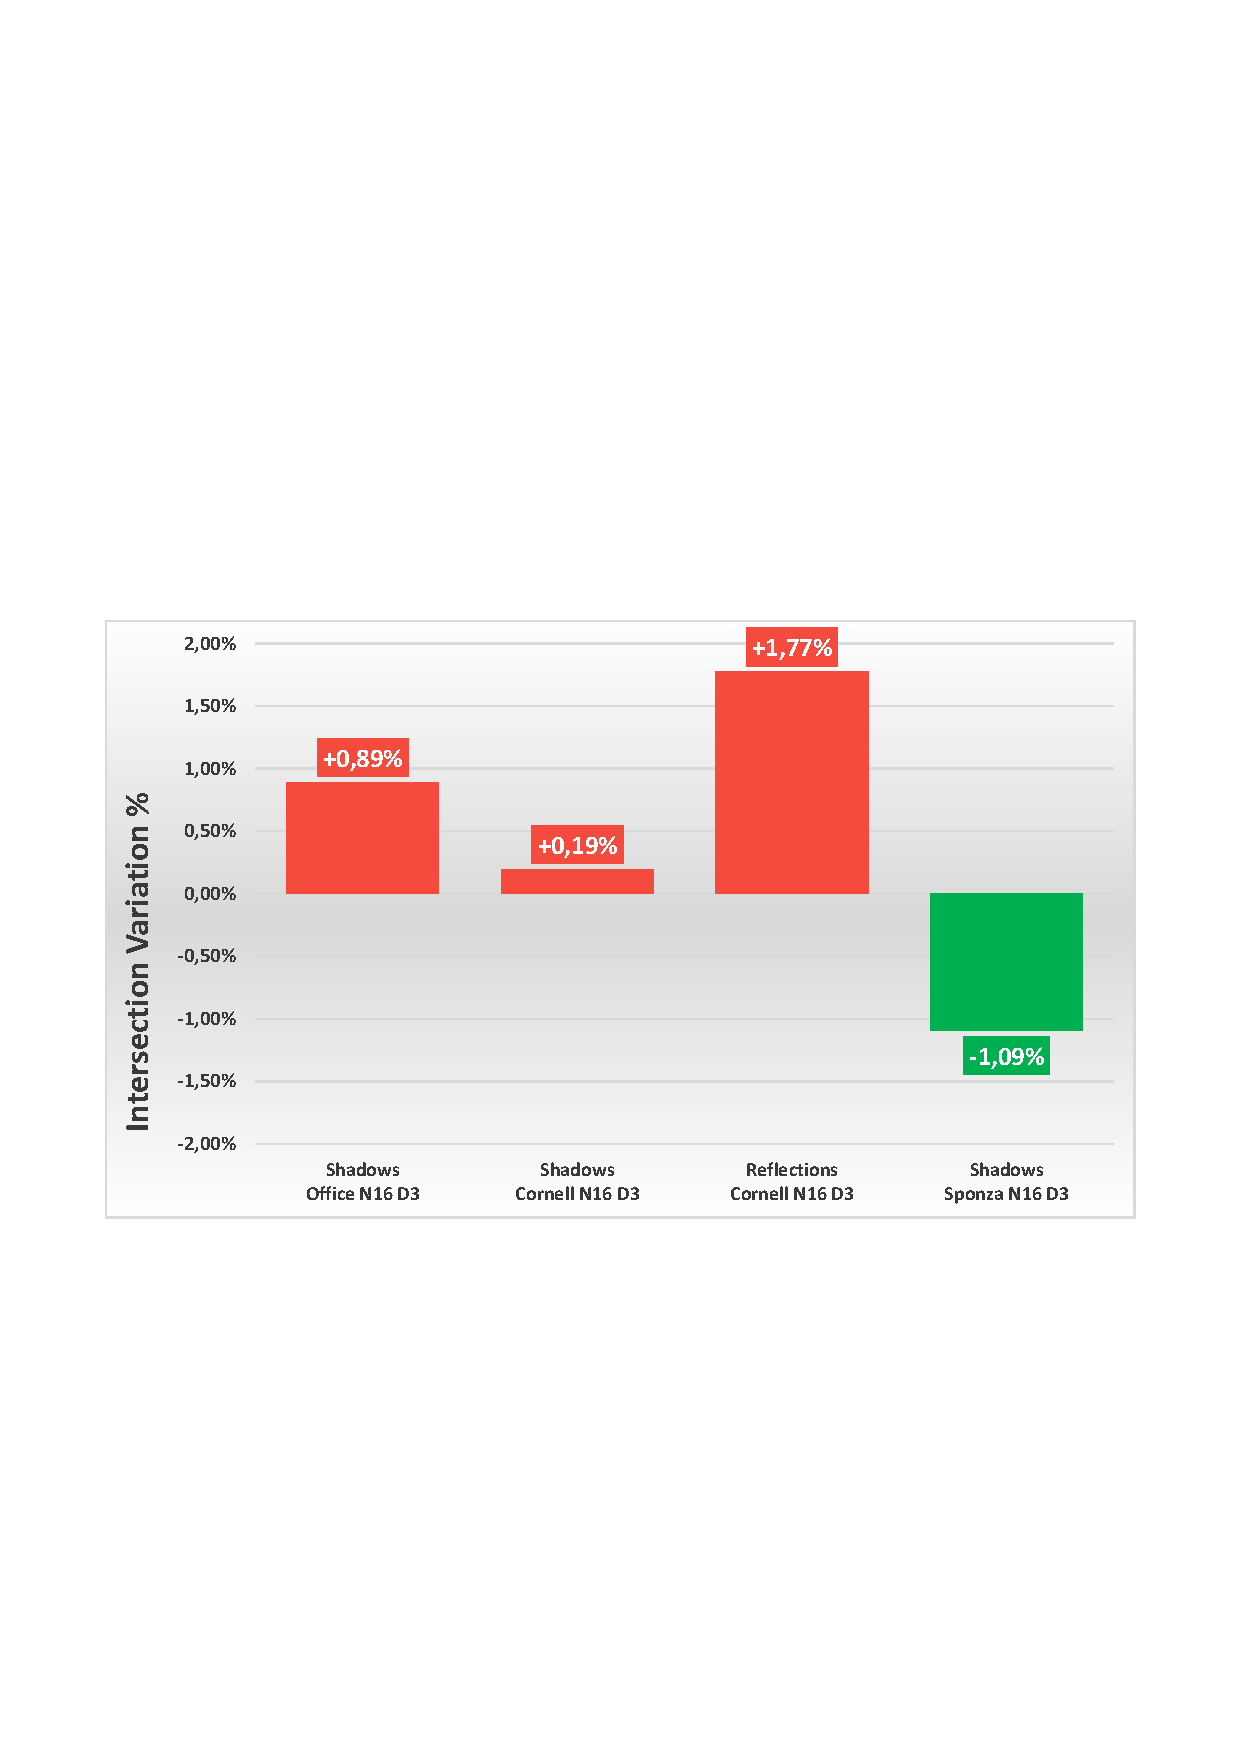
\includegraphics[width=0.70\textwidth]{Images/Chart_Comparison_N8_D2_N16_D3}
    \label{fig:comparison-results-d8-n2-d16-n3}
    \caption{Configuration Comparison between Node Subdivision 8 with Hierarchy Depth 2 and Node Subdivision 16 with Hierarchy Depth 3.}
    \end{center}
\end{figure}

For this set of tests we used a node subdivision of 16 and a hierarchy depth of 3. This means that every node in the upper levels of the hierarchy consists of 16 nodes in the level directly below. We compared this configuration with the baseline configuration of node subdivision of 8 and hierarchy depth of 2.

\subsubsection{Office}

Once more, increasing the depth of the hierarchy outperforms the RAH algorithm (see Table~\ref{table:office-d16-n3-results}). We compute 62.59\% less intersections than RAH on this scene and 97,25\% less than a brute force approach. There is an increase of 0.70\% when compared to the baseline (from 1.86\% to 2.75\%) (see Figure~\ref{fig:comparison-results-d8-n2-d16-n3}).

\subsubsection{Cornell}

For the Cornell scene we compute 29,62\% less intersections overall (shadow and reflection rays combined) than the RAH algorithm and 89,90\% less than the brute force approach (see Table~\ref{table:cornell-d16-n3-results}). When we compare these results with the baseline configuration we get an increase of 0.13\%, from 7.45\% to 7.65\% for shadow rays and from 9.46\% to 11.24\% for reflection rays (see Figure~\ref{fig:comparison-results-d8-n2-d16-n3}). This continues the trend seen in previous test results.

\subsubsection{Sponza}

In the Sponza scene we compute 72,17\% less intersection tests than RAH and 98,72\% than the brute force approach (see Table~\ref{table:sponza-d16-n3-results}). The number of intersection tests was reduced once again, going from the baseline 2.38\% to 1.28\% (see Figure~\ref{fig:comparison-results-d8-n2-d16-n3}). Since we increased the depth from the previous configuration it is natural that the trend for a decrease in intersection tests remains until we reach the break point.

%%%%%%%%%%%%%%%%%%%%%%%%%%%%%%%%%%%%%%%%%%%%%%%%%%%%%%%%%%%%%%%%%%%%%%%%%%%%%%%%%%%%%%%%%%%%%%%%%%%%%%%%%%%%%%%%%%%%%%%%%%%%%%%%%%

\pagebreak
\subsection{Hierarchy Traversal Results - Subdivision 16 Depth 4}

\subsubsection{Office}

% Office Discussion

Comparing our algorithm with the RAH algorithm we can see that our algorithm computes 39,18\% less intersections than RAH on this scene. 97,87\% less than a brute force approach (see Table~\ref{table:office-d16-n4-results} and Table~\ref{table:results-d16-n4}).

% Office Table and Figure
    
\begin{figure}[!htb]
    \begin{minipage}{0.25\linewidth}
        \centering
        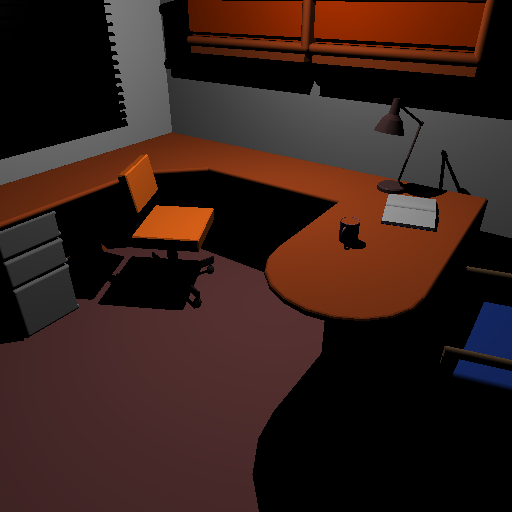
\includegraphics[width=4.0cm]{Images/Office_Preview}
        \captionof{figure}{\textsc{Office}}
    \end{minipage}
    \begin{minipage}{0.725\linewidth}
        \centering
        \fontencoding{T1}
        \fontseries{m}
        \fontshape{sc}
        \fontsize{8}{10}
        \selectfont
        \begin{tabular}[h]{l|rrrr}
            \multicolumn{1}{c|}{\textsc{Office}} & \textsc{Level 4} & \textsc{Level 3} & \textsc{Level 2} & \textsc{Level 1}\\
            \hline
            \emph{RAH Algorithm} & & \\
            \hline
            \quad \# Sh Intersections  & 145232	& 2323712   & 36017536	& 412453440	\\
            \quad \# Sh Misses         & 0		& 72616		& 10239196	& 398662535	\\
            \quad \# Sh Hits           & 145232	& 2251096	& 25778340	& 13790905	\\
            \hline
            \emph{Our Algorithm} & & \\
            \hline
            \quad \# Sh Intersections  & 145232	& 2323712	& 23351216	& 119524928	\\
            \quad \# Sh Misses         & 0		& 864261	& 15880908	& 112848037	\\
            \quad \# Sh Hits           & 145232	& 1459451	& 7470308	& 6676891	\\
        \end{tabular}
        \label{table:office-d16-n4-results}
        \captionof{table}{\textsc{Office} Division 16 Depth 4 Test Results.}
    \end{minipage}
\end{figure}

\subsubsection{Cornell}

% Cornel Discussion

Comparing our algorithm with the RAH algorithm we can see that our algorithm computes 26,47\% less intersections than RAH on this scene. 91,17\% less than a brute force approach (see Table~\ref{table:cornell-d16-n4-results} and Table~\ref{table:results-d16-n4}).

% Cornell Table and Figure

\begin{figure}[!htb]
    \begin{minipage}{0.25\linewidth}
        \centering
        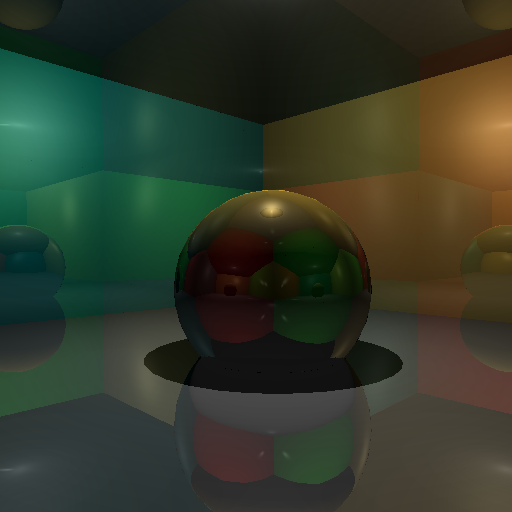
\includegraphics[width=4.0cm]{Images/Cornell_Preview}
        \captionof{figure}{\textsc{Cornell}}
    \end{minipage}
    \begin{minipage}{0.725\linewidth}
        \centering
        \fontencoding{T1}
        \fontseries{m}
        \fontshape{sc}
        \fontsize{8}{10}
        \selectfont
        \begin{tabular}[h]{l|rrrr}
            \multicolumn{1}{c|}{\textsc{Office}} & \textsc{Level 4} & \textsc{Level 3} & \textsc{Level 2} & \textsc{Level 1}\\
            \hline
            \emph{RAH Algorithm} & & \\
            \hline
            \quad \# Sh Intersections   & 3168		& 50688		& 760128	& 7732000	\\
            \quad \# Sh Misses          & 0		    & 3180		& 276878	& 6808346	\\
            \quad \# Sh Hits            & 3168		& 47508		& 483250	& 923654	\\
            & & \\
            \quad \# Re Intersections   & 6336		& 101376	& 1622016	& 23053680	\\
            \quad \# Re Misses          & 0	        & 0	        & 181161	& 20614507	\\
            \quad \# Re Hits            & 6336		& 101376	& 1440855	& 2439173	\\
            \hline
            \emph{Our Algorithm} & & \\
            \hline
            \quad \# Sh Intersections   & 3168	    & 50688		& 498352	& 2577680	\\
            \quad \# Sh Misses          & 0		    & 19541		& 337247	& 1856187	\\
            \quad \# Sh Hits            & 3168		& 31147	    & 161105	& 721493	\\
            & & \\
            \quad \# Re Intersections   & 6336		& 101376	& 1620432	& 11466336	\\
            \quad \# Re Misses          & 0		    & 99	    & 903786	& 9374256	\\
            \quad \# Re Hits            & 6336		& 101277	& 716646	& 2092080	\\            
        \end{tabular}
        \label{table:cornell-d16-n4-results}
        \captionof{table}{\textsc{Cornell} Division 16 Depth 4 Test Results.}
    \end{minipage}
\end{figure}

\subsubsection{Sponza}

% Sponza Discussion

Comparing our algorithm with the RAH algorithm we can see that our algorithm computes 35,86\% less intersections than RAH on this scene. 97,62\% less than a brute force approach (see Table~\ref{table:sponza-d16-n4-results} and Table~\ref{table:results-d16-n4}).

% Sponza Table and Figure

\begin{figure}[!htb]
    \begin{minipage}{0.25\linewidth}
        \centering
        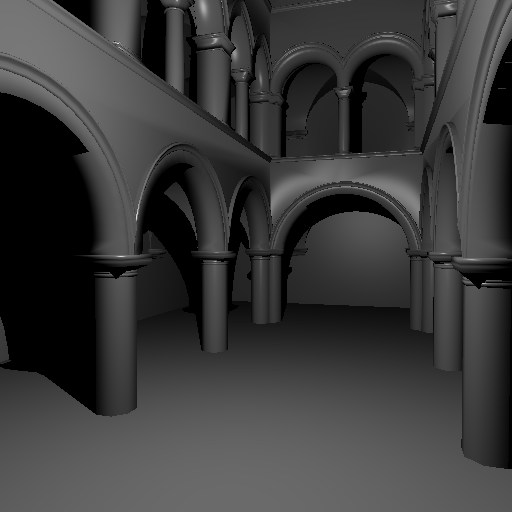
\includegraphics[width=4.0cm]{Images/Sponza_Preview}
        \captionof{figure}{\textsc{Sponza}}
    \end{minipage}
    \begin{minipage}{0.725\linewidth}
        \centering
        \fontencoding{T1}
        \fontseries{m}
        \fontshape{sc}
        \fontsize{8}{10}
        \selectfont
        \begin{tabular}[h]{l|rrrr}
            \multicolumn{1}{c|}{\textsc{Office}} & \textsc{Level 4} & \textsc{Level 3} & \textsc{Level 2} & \textsc{Level 1}\\
            \hline
            \emph{RAH Algorithm} & & \\
            \hline
            \quad \# Sh Intersections   & 265800	& 4252800	& 66981600	& 554494192	\\
            \quad \# Sh Misses          & 0		    & 66450		& 32325713	& 544455870	\\
            \quad \# Sh Hits            & 265800	& 4186350	& 34655887	& 10038322	\\
            & & \\
            \hline
            \emph{Our Algorithm} & & \\
            \hline
            \quad \# Sh Intersections   & 265800	& 4252800	& 29037376	& 102667568	\\
            \quad \# Sh Misses          & 0	        & 2437964   & 22620653	& 97483134	\\
            \quad \# Sh Hits            & 265800	& 1814836	& 6416723	& 5184434	\\
        \end{tabular}
        \label{table:sponza-d16-n4-results}
        \captionof{table}{\textsc{Sponza} Division 16 Depth 4 Test Results.}
    \end{minipage}
\end{figure}

\subsection{Hierarchy Traversal Discussion - Subdivision 16 Depth 4}

% Comparison Table

\begin{table}[!htb]
    \begin{center}
    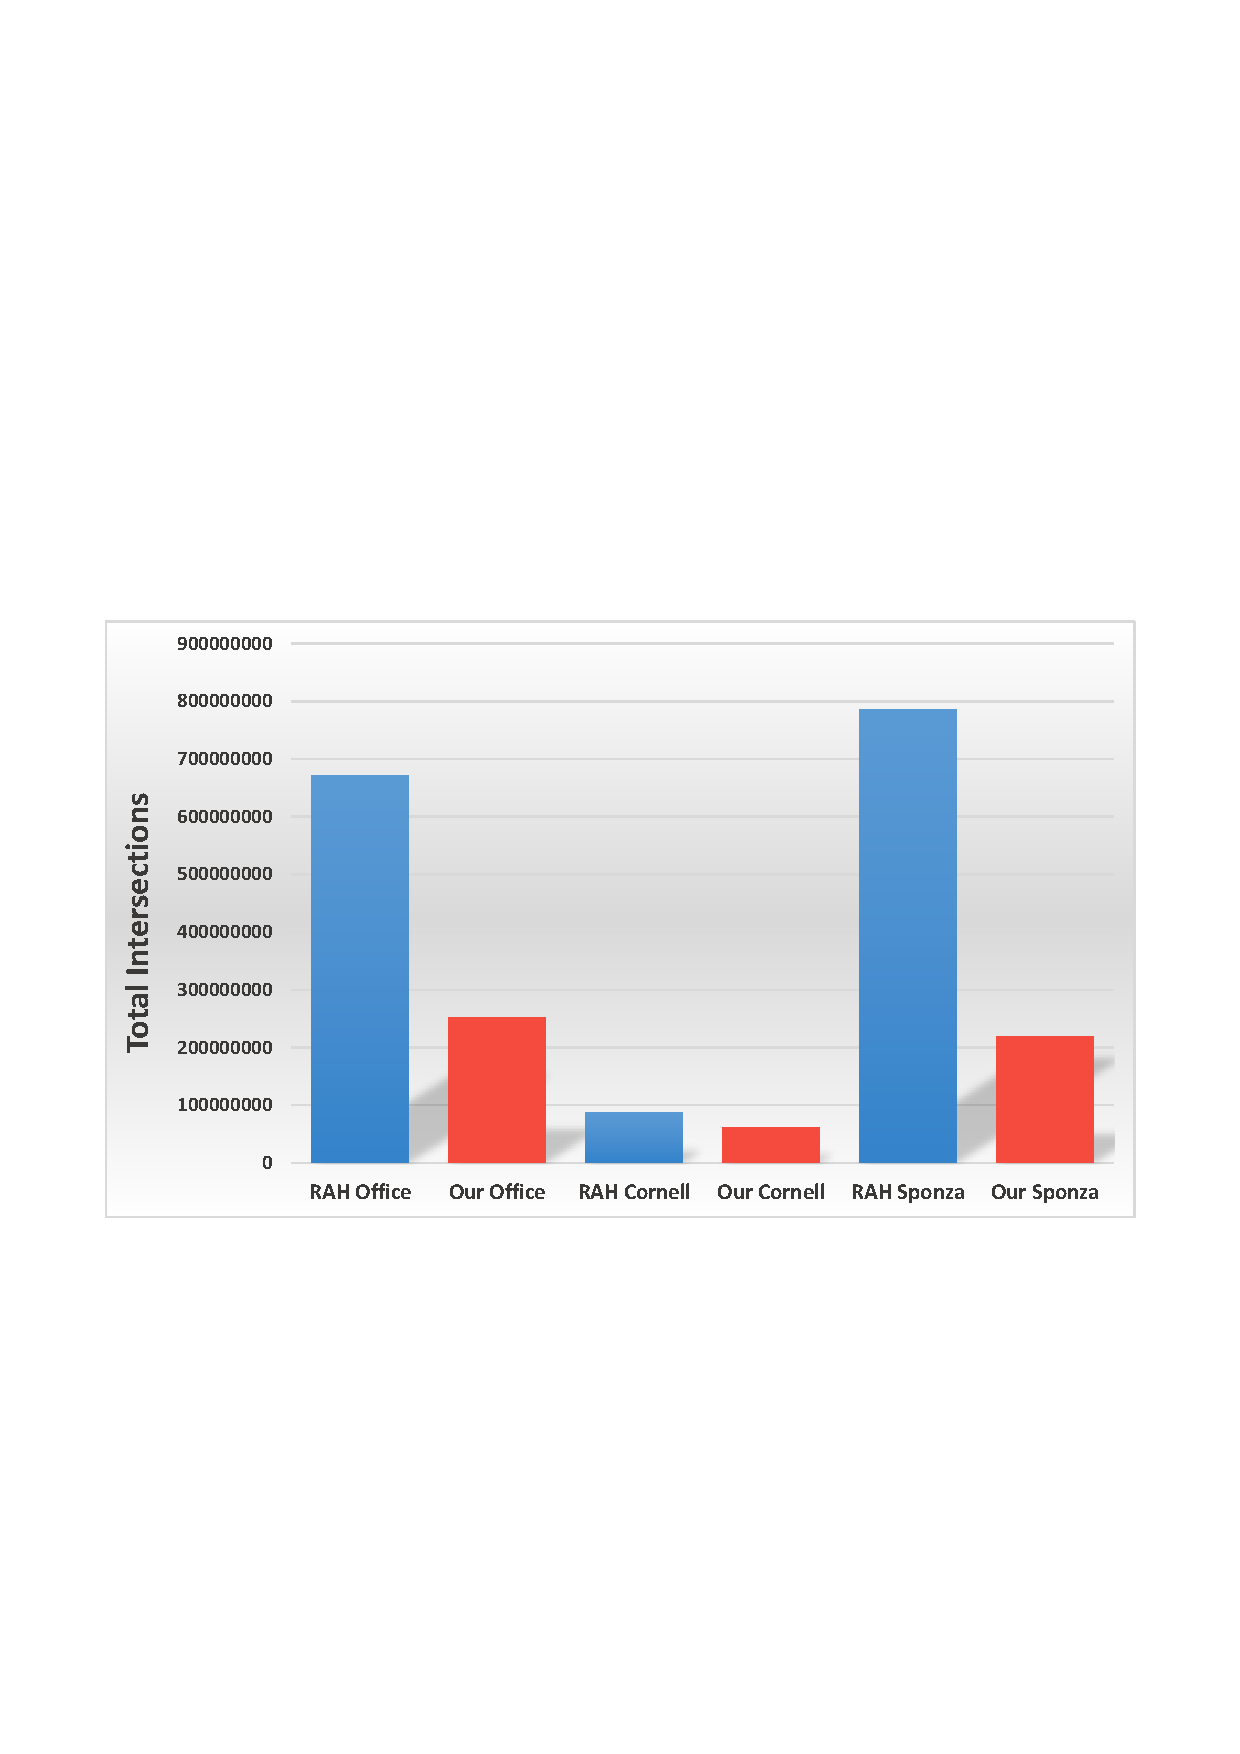
\includegraphics[width=0.85\textwidth]{Images/Chart_N16_D4}
    \vskip 2em
    \fontencoding{T1}
    \fontseries{m}
    \fontshape{sc}
    \fontsize{8}{10}
    \selectfont
    \begin{tabular}{l|rrrrrr}
    & \multicolumn{2}{c}{\textsc{Office}} & \multicolumn{2}{c}{\textsc{Cornell}} & \multicolumn{2}{c}{\textsc{Sponza}} \\
    \textsc{Algorithm} & \textsc{Total \# isect} & \textsc{Relative \%} & \textsc{Total \# isect} & \textsc{Relative \%} & \textsc{Total \# isect} & \textsc{Relative \%} \\
        \hline
        \emph{Brute Force}     & 9133132168         & 100\%           & 606911976         & 100\%           & 17058578850         & 100\% \\
        \emph{RAH Algorithm}   & 671594400			& 7.35\%          & 87134624		  & 14.36\%         & 786607544		      & 4.61\% \\
        \emph{Our Algorithm}   & \textbf{252175344} & \textbf{2.76\%} & \textbf{61341536} & \textbf{10.11\%} & \textbf{219174488} & \textbf{1.28\%} \\
    \end{tabular}
    \end{center}
    \caption{\label{table:results-d16-n4}
    \small\textsc{Office} (251546 shadow rays), \textsc{Cornell} (242015 shadow \& 524288 reflection rays), \textsc{Sponza} (256713 shadow rays) rendering performance  using node subdivision 16 and hierarchy depth 4.}
\end{table}

\begin{figure}[!htb]
    \begin{center}
    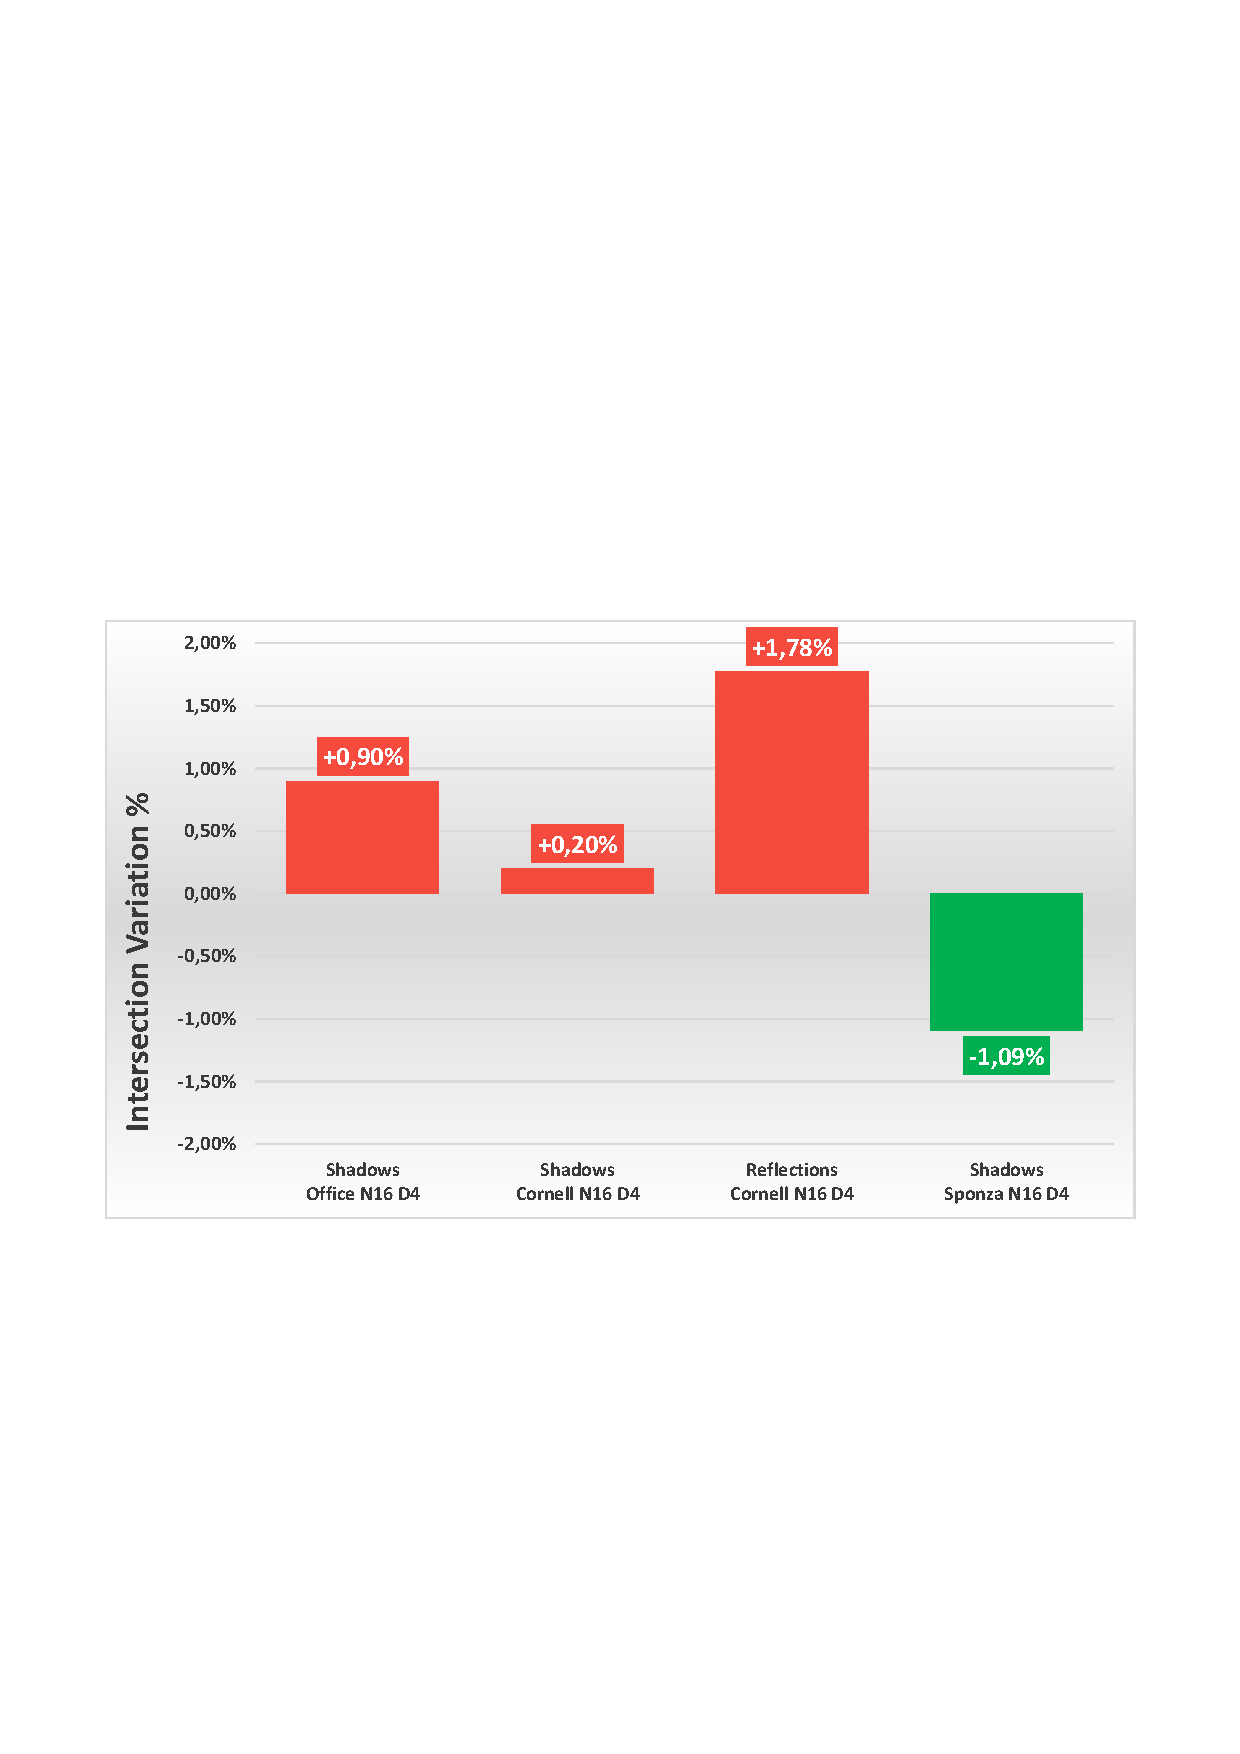
\includegraphics[width=0.70\textwidth]{Images/Chart_Comparison_N8_D2_N16_D4}
    \label{fig:comparison-results-d8-n2-d16-n4}
    \caption{Configuration Comparison between Node Subdivision 8 with Hierarchy Depth 2 and Node Subdivision 16 with Hierarchy Depth 4.}
    \end{center}
\end{figure}

For this set of tests we used a node subdivision of 16 and a hierarchy depth of 3. This means that every node in the upper levels of the hierarchy consists of 16 nodes in the level directly below. We compared this configuration with the baseline configuration of node subdivision of 8 and hierarchy depth of 2.

\subsubsection{Office}

For the final configuration the Office scene calculated less intersections the RAH algorithm (see Table~\ref{table:office-d16-n4-results}). We compute 62.45\% less intersections than RAH on this scene and 97,24\% less than a brute force approach. There is yet another increase of 0.70\% when compared to the baseline (from 1.86\% to 2.75\%) (see Figure~\ref{fig:comparison-results-d8-n2-d16-n3}). 

\subsubsection{Cornell}

For the final test for the Cornell scene we compute 29,60\% less intersections overall (shadow and reflection rays combined) than the RAH algorithm and 89,89\% less than the brute force approach (see Table~\ref{table:cornell-d16-n4-results}). When we compare these results with the baseline configuration we get an increase of 0.13\%, from 7.45\% to 7.66\% for shadow rays and from 9.46\% to 11.25\% for reflection rays (see Figure~\ref{fig:comparison-results-d8-n2-d16-n4}).

\subsubsection{Sponza}

For the final test using the Sponza scene we computed 72,14\% less intersection tests than RAH and 98,68\% than the brute force approach (see Table~\ref{table:sponza-d16-n4-results}). The number of intersection tests was reduced once again, going from the baseline 2.38\% to 1.28\% (see Figure~\ref{fig:comparison-results-d8-n2-d16-n4}). We increased the depth from the previous configuration but we got a small increase in the intersection tests. This indicates that the previous configuration is the break point after which increasing the depth stops yielding benefits for this scene.

%%%%%%%%%%%%%%%%%%%%%%%%%%%%%%%%%%%%%%%%%%%%%%%%%%%%%%%%%%%%%%%%%%%%%%%%%%%%%%%%%%%%%%%%%%%%%%%%%%%%%%%%%%%%%%%%%%%%%%%%%%%%%%%%%%

\subsection{Frame Rate Results}

\subsubsection{Office}

\subsubsection{Cornell}

\subsubsection{Sponza}

%%%%%%%%%%%%%%%%%%%%%%%%%%%%%%%%%%%%%%%%%%%%%%%%%%%%%%%%%%%%%%%%%%%%%%%%%%%%%%%%%%%%%%%%%%%%%%%%%%%%%%%%%%%%%%%%%%%%%%%%%%%%%%%%%%

\subsection{Test Results Global Discussion}

For the Office scene the tests indicated that the optimal configuration is in fact the baseline configuration used, using node subdivision of 8 and hierarchy depth of 2. However this is reliant on the hashing function used, which means that if a better hashing function is used the optimal configuration may be different. 

For the Cornell scene there was always an increase for every configuration when compared with the baseline configuration. However this increase was more significant for the reflection rays. This is due to the fact that reflection rays are much less coherent than shadow rays, which leads to bigger nodes when combining such rays. Much like the shadow rays however using better hashing functions can mitigate this effect.

Finally for the Sponza scene we noticed a reverse trend compared to the remaining scenes. This is due to the fact that the scene itself isn't subdivided into several objects, making the use of bounding spheres useless. As such, only the higher levels of the hierarchy were culling the number of potential intersection tests, which means that as we increased the hierarchy's depth this mitigation effect would be increased until we reached a certain break point, like it was noted before. Since this scene is an outlier however it is safe to assume if it was subdivided into several objects, much like the Office scene, the optimal configuration would be the baseline configuration used for the tests. 